\chapter{Upscaling global carbon fluxes}
\renewcommand{\headrulewidth}{0pt}
\lhead[\thepage]{\leftmark}
\rhead[\leftmark]{\thepage}
\cfoot[]{}

\section{Introduction}

\begin{figure}[tbh!]
    \centering
    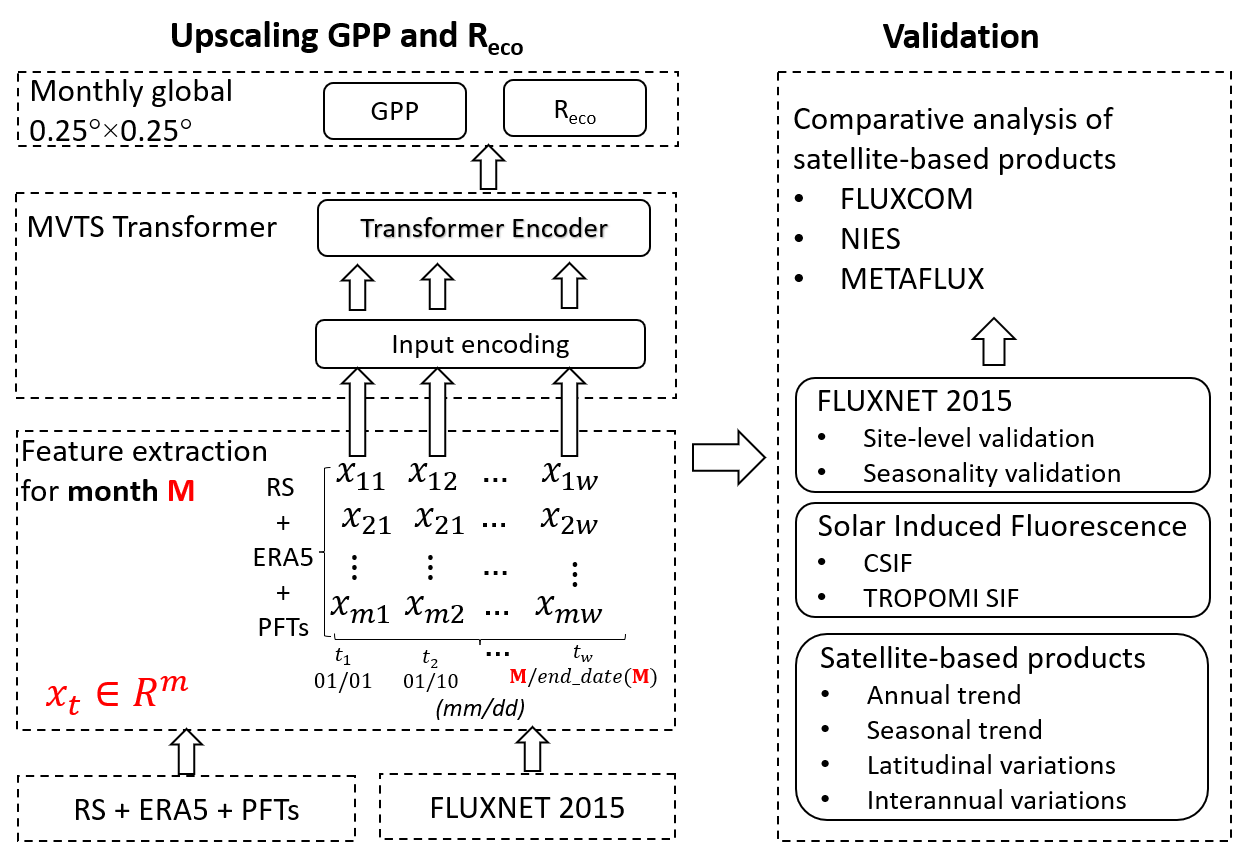
\includegraphics[width=\textwidth]{figs/chap6/workflow.png}
    \caption[Schemantic workflow of our FluxFormer methodology]{Schemantic workflow of our FluxFormer methodology}
    \label{fig:chap6_fig1}
\end{figure}

\section{Methods}
\subsection{Input data}

\subsubsection*{FLUXNET 2015}
The FLUXNET 2015 dataset \citep{pastorello2020fluxnet2015} serves as the groundtruth for carbon fluxes in the transformer model in this study. Monthly GPP and RECO data were extracted from the dataset tier 1 of FLUXNET 2015, encompassing data from 206 sites. We filtered out records with a quality control value of less than 80\% for measured and good-quality gap-fill data. Relying solely on quality control values is reported to be insufficient for obtaining qualified data due to inconsistencies in the differences between GPP, RECO, and NEE \citep{zeng2020global, tramontana2016predicting}. Following the approach of \citep{zeng2020global}, we also excluded records with an absolute difference between GPP-RECO and NEE larger than 0.1 gC $m^{-2} d^{-1}$. The distribution of FLUXNET 2015 sites is unbalanced across climate zones, particularly in tropics and semi-arid areas, despite the highest GPP values in tropical regions (Amazonia, Central Africa, and Southeast Asia) \citep{chen2017regional}. Additionally, semi-arid regions are considered important drivers of the global carbon cycle \citep{poulter2014contribution}. Therefore, only the most recent data up to 3 years for each site was used to balance the representation of each site during the training of the transformer model. \par
\subsubsection*{Remote sensing data}
For the remote sensing data, we employed version 2 of the global leaf area index (LAI) and fraction of absorbed photosynthetically active radiation (FAPAR) datasets, generated using the algorithm proposed by \citep{verger2014near}. These datasets can be accessed through the Copernicus Global Land Service, providing a 1 km spatial resolution for every 10 days spanning from 1999 to 2019. The remote sensing data utilized in this study is in line with the approach presented in \citep{zeng2020global}. The latitude boundary of this dataset ranges from -60°S to 80°N. \par
\subsubsection*{Meteorological data}
For meteorological data, we employed specific variables from the ERA5 reanalysis product \citep{hersbach2020era5}, including 2-meter air temperature (T2M), surface short-wave (solar) radiation downwards (SSRD), vapor pressure deficit (VPD), total precipitation (TP), and evaporation (E). As VPD is not directly available in the original dataset, we estimated it using the relationship between saturated vapor pressure (SVP) and actual vapor pressure (AVP): VPD = SVP - AVP, based on 2-meter air and dewpoint temperature. The original spatial resolution of ERA5 data is 0.25° × 0.25° and was obtained from the Copernicus Climate Change Service (C3S) Climate Data Store (CDS). \par

\subsubsection*{Plant function types}
The PFTs dataset employed in this study, denoted as PFT v2.0.8 and obtained from \citep{harper202229}, spans the period from 1992 to 2020. It provides the specific percentage cover of 14 PFTs for each pixel at a 300m resolution. The annual dataset comprises 14 layers, with pixel values at 300m resolution indicating the percentage cover (ranging from 0\% to 100\%) for each of the 14 PFTs. This updated PFTs dataset is considered a more accurate representation of PFT distributions as it relies on high-resolution, peer-reviewed mapping of specific vegetation classes to refine global assumptions about PFT fractions \citep{harper202229}. Regional updates in PFT fractions are anticipated to enhance carbon fluxes estimation. The complete set of PFTs includes bare soil, built areas, water bodies, snow and ice, natural grasses, managed grasses (i.e., herbaceous cropland), broadleaved deciduous trees, broadleaved evergreen trees, needleleaved deciduous trees, needleleaved evergreen trees, broadleaved deciduous shrubs, broadleaved evergreen shrubs, needleleaved deciduous shrubs, and needleleaved evergreen shrubs. The dataset can be accessed from the CEDA archive at https://catalogue.ceda.ac.uk/uuid/26a0f46c95ee4c29b5c650b129aab788.\par

\subsection{Multivariate Time Series Transformer Framework}
Figure \ref{fig:chap6_fig1} illustrates the overall workflow of our FluxFormer methodology to upscale GPP and RECO from remote sensing data, and PFTs data. We utlized the original Multivariate Time Series MVTS Transformer model which is transformer-based framework proposed by \citep{zerveas2021transformer} which contains an input encoding layer with learnable positional encoding and a Transformer Encoder \citep{vaswani2017attention}. MVTS Transformer achieved good performance on supervised and unsupervised regression task based on multivariate time series representation even with limited training samples.  \par
In order train the MVTS Transformer, First, we extracted the remote sensing data, meteorological data and PFTs for each monthly record from FLUXNET 2015 dataset. Then the extracted data is formed to feed to the deep learning model. In particular, for a specific month \textbf{M}, each traing sample $\mathbf{X} \in \mathbb{R}^{w\times n}$ where \textit{w} is the lengths of timeseries for month \textbf{M} $\textit{w} = 3\times \textbf{M}$ as we have 3 remote sensing products per month and \textit{m} is the number of different variables  $\textit{m} = 21$ 2 remote sensing varibales (LAI and FAPAR), 5 meteorological variables (T2M, SSRD, VPD, TP, E) and 14 PFTs variables, constitutes a sequence of \textit{w} feature vectors $\mathbf{x}\textsubscript{t} \in \mathbb{R}^{m}: \mathbf{X} \in \mathbb{R}^{w\times n} = [\mathbf{x}\textsubscript{1},\mathbf{x}\textsubscript{1}, \dots, \mathbf{x}\textsubscript{w}]$ is a multivariate timeseries of length w and m different variables. \par

\subsection{Training setup}
In order to train the model, we randomly selected 80\% of the monthly data to train the model and use the rest 20\% for the validation. We train 12 model for 12 months. \par
\subsection{Validation}
To evaluate our product's quality, we performed a comparative analysis against other remote sensing-based products, including FLUXCOM \citep{jung2019fluxcom}, NIES \citep{zeng2020global}, and MetaFlux \citep{nathaniel2023metaflux}. Initially, we assessed the correlation of monthly FLUXNET 2015 GPP and RECO values with the corresponding data from these products at the FLUXNET sites. Subsequently, we conducted a seasonality examination using FLUXNET 2015 and Solar-Induced Fluorescence (SIF) from CSIF \citep{zhang2018global} (accessible at https://fgshare.com/articles/dataset/CSIF/6387494) and TROPOMI SIF \citep{kohler2018global} (retrievable from ftp://fluo.gps.caltech.edu/data/tropomi/). Finally, we examined the interannual trends and variations of our products in comparison to FLUXCOM, NIES, and MetaFlux. To assess interannual trends, we computed the annual global mean GPP and RECO, scaling the global average fluxes with the total global land area (122.4 million $km^{2}$) from \citep{friedl2010modis}, as recommended by \citep{jung2020scaling} for consistent global area representation across all products. We utilized the slope of the linear regression line and p-value to indicate the annual trends and statistical significance of the trends in GPP and RECO. For the assessment of interannual variations, we calculated the Interannual Variability (IAV) at the pixel level by determining the standard deviation divided by the mean of annual fluxes. \par

\section{Data records}
\begin{figure}[p]
    \centering
    \begin{subfigure}{\textwidth}
      \centering
      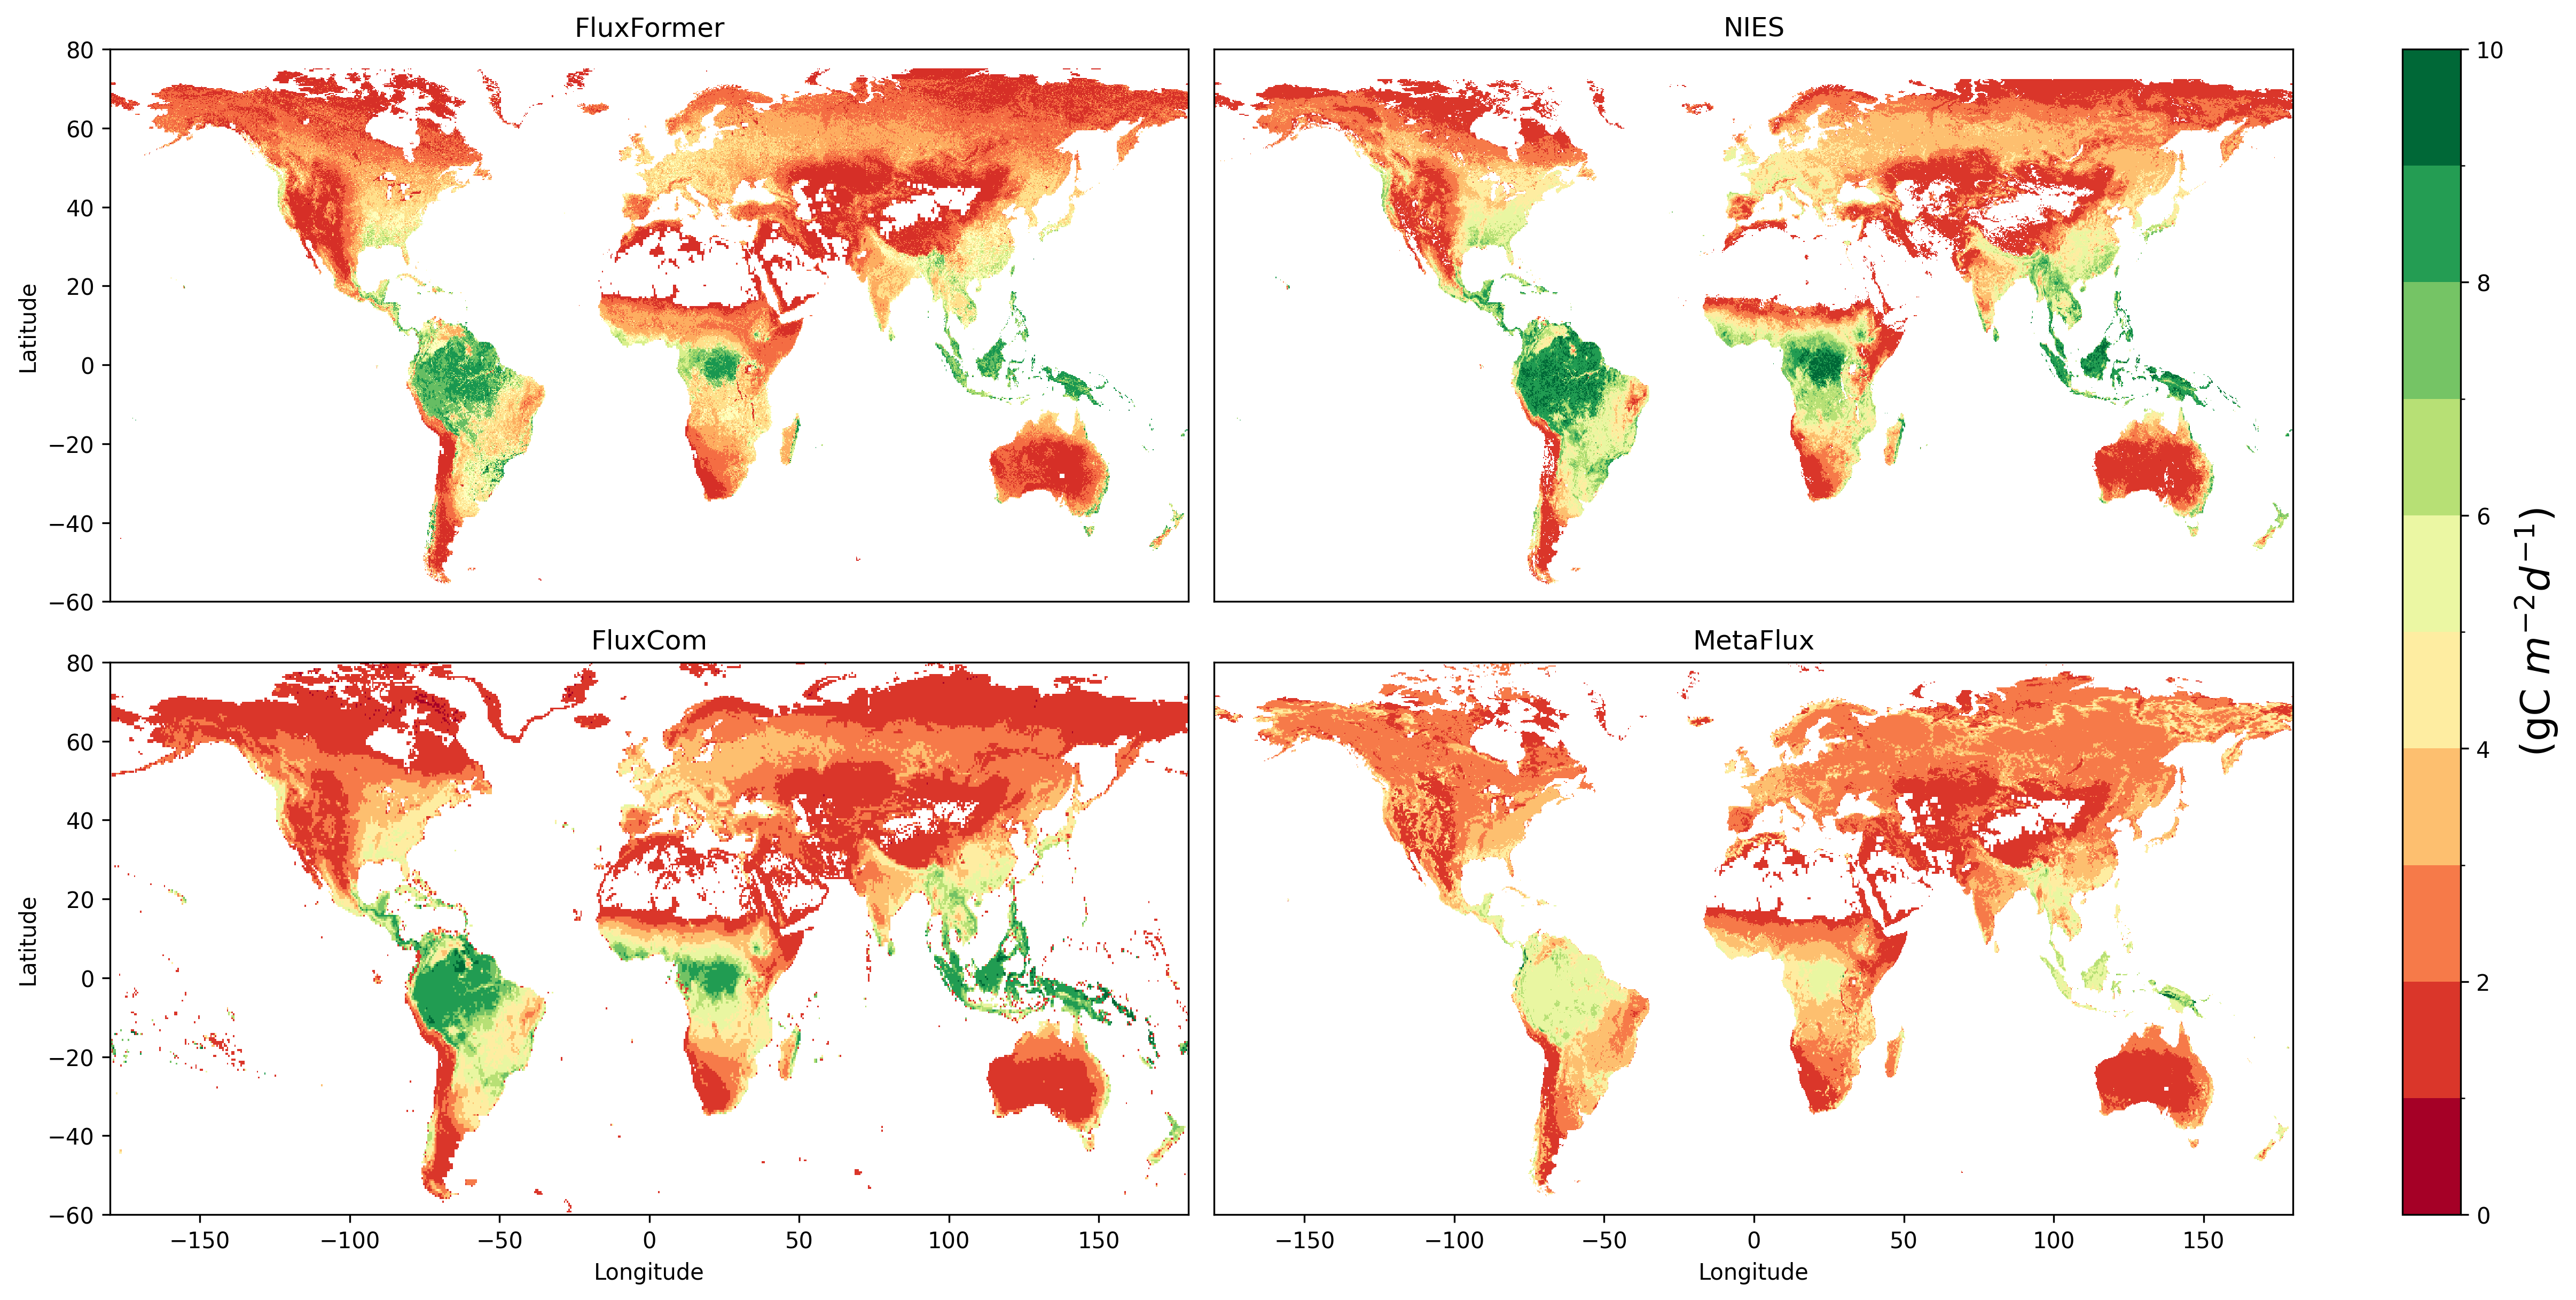
\includegraphics[width=\textwidth]{figs/chap6/GPP_2017_mean.png}
      \caption{GPP}
      \label{fig:chap6_fig2a}
    \end{subfigure}

    \begin{subfigure}{\textwidth}
      \centering
      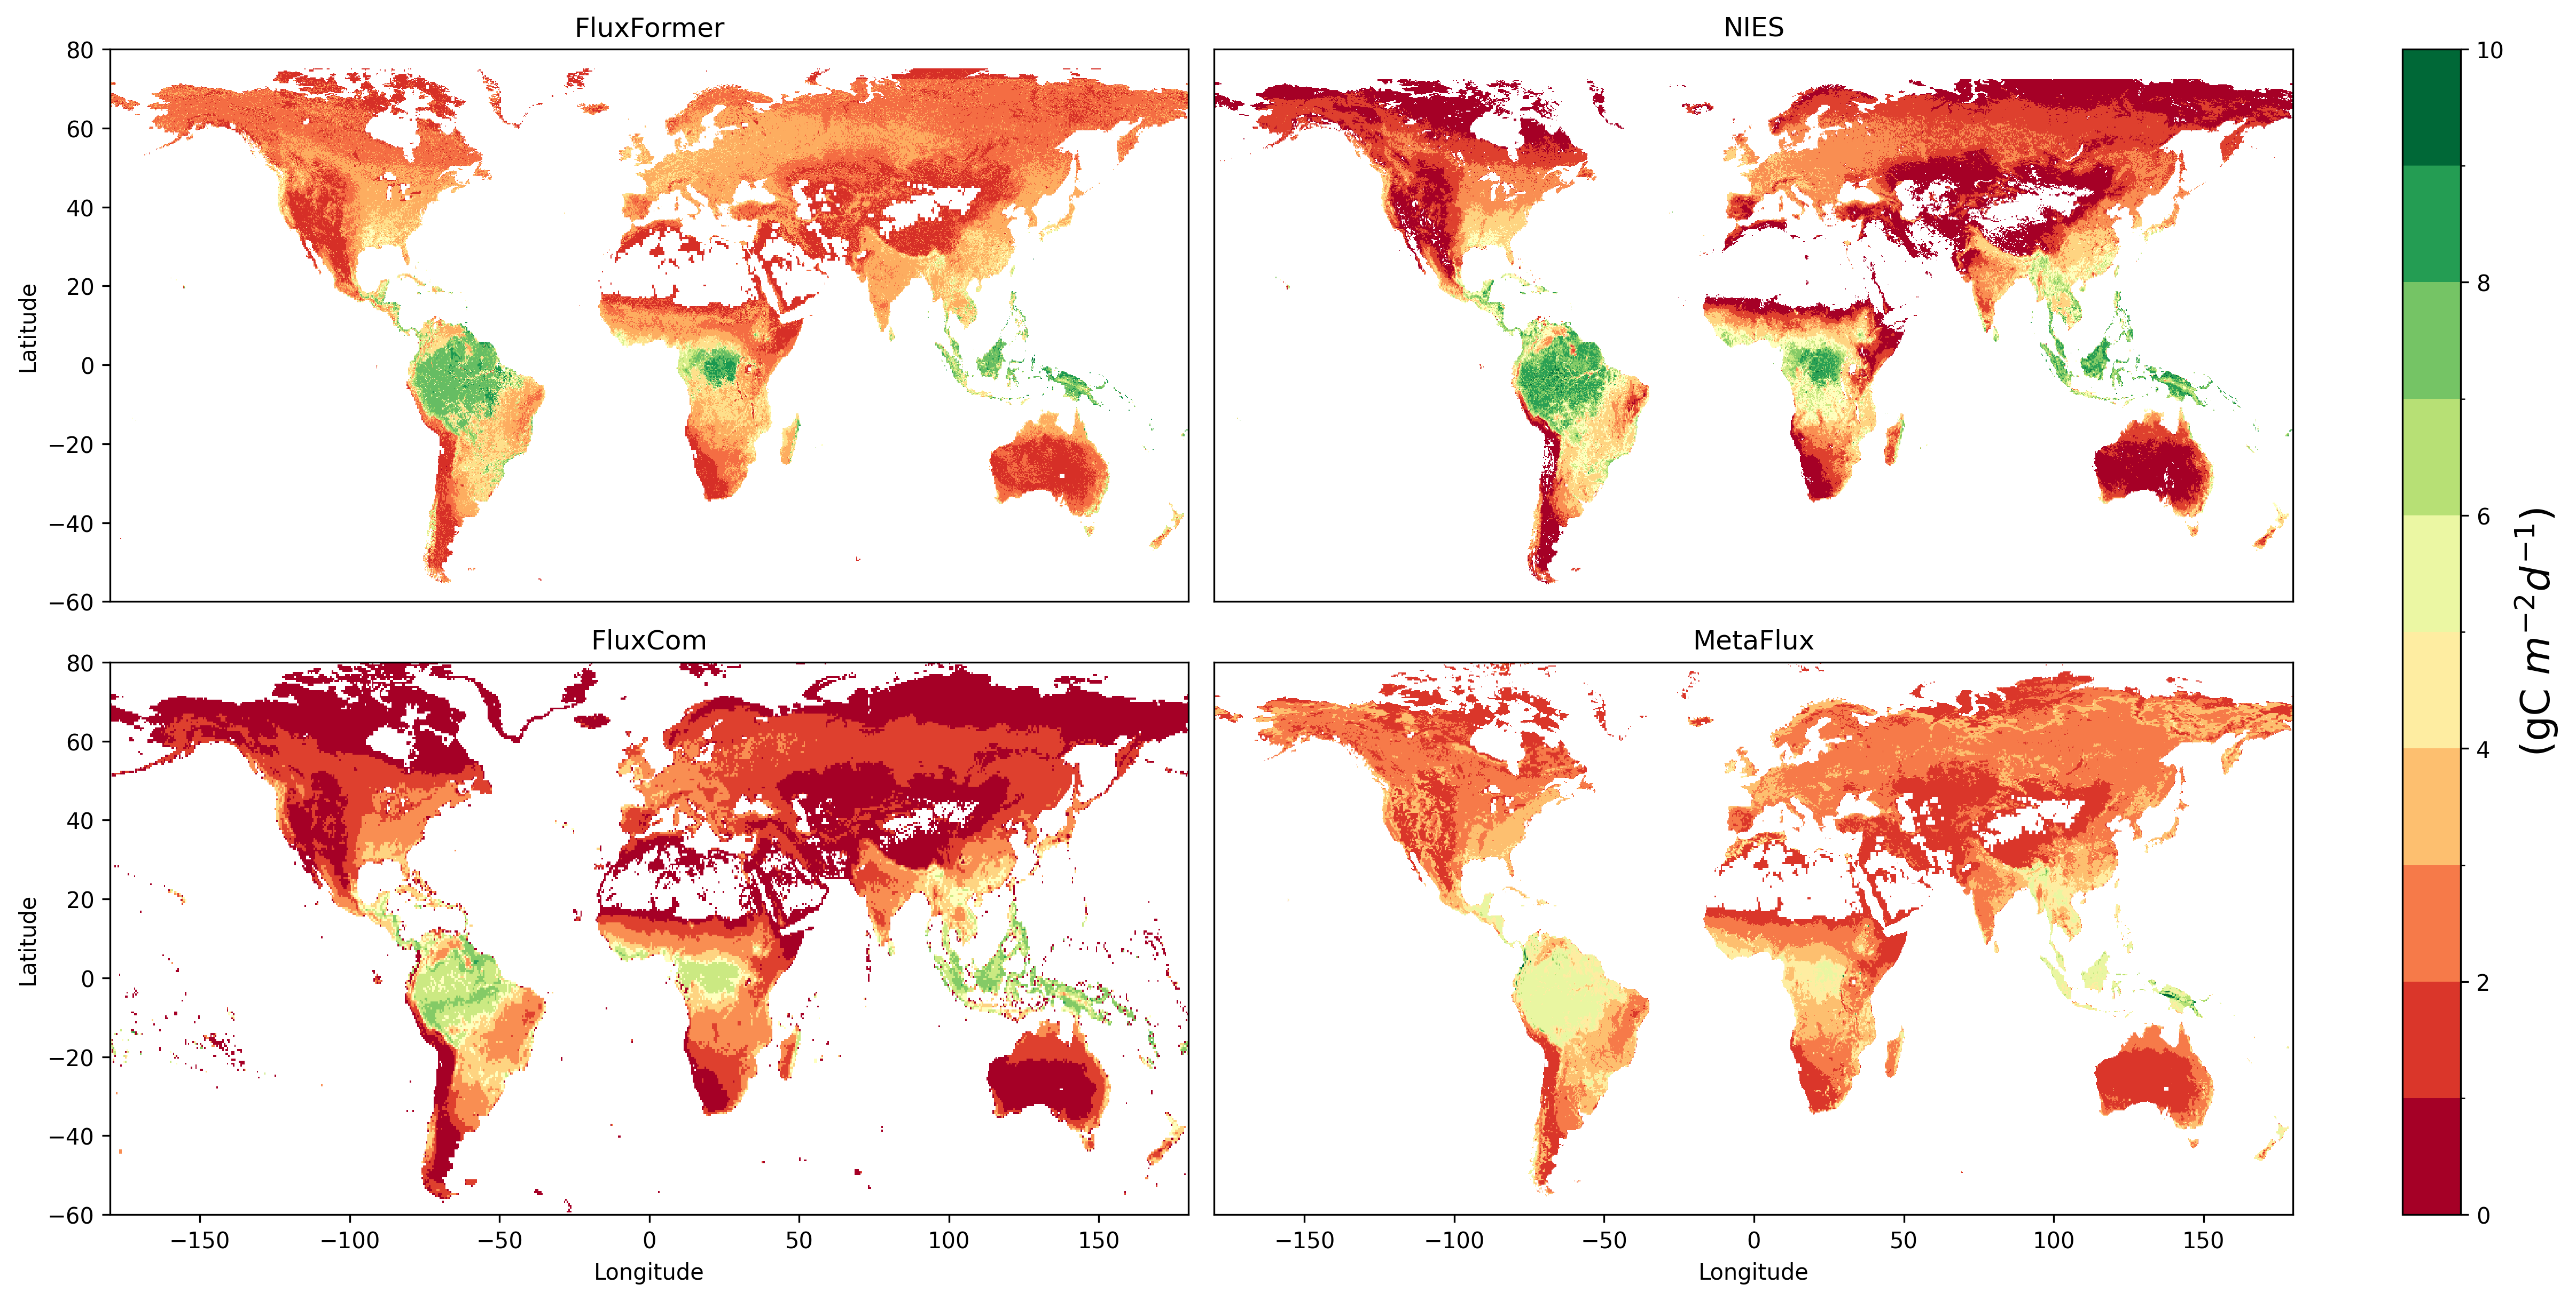
\includegraphics[width=\textwidth]{figs/chap6/RECO_2017_mean.png}
      \caption{RECO}
      \label{fig:chap6_fig2b}
    \end{subfigure}
    \caption[Validation with FLUXNET 2015]{Validation with FLUXNET 2015: GPP (a) RECO (b)}
    \label{fig:chap6_fig2}
\end{figure}

\section{Technical validation}
\subsection{Validation with FLUXNET 2015}
\subsubsection*{Site-level validation}
As depicted in Figures \ref{fig:chap6_fig3a} and \ref{fig:chap6_fig3b}, our product exhibits the highest correlation with FLUXNET 2015 for both GPP and RECO data ($R = 0.883$ for GPP and $R = 0.86$ for RECO), whereas MetaFlux shows the lowest correlation with FLUXNET 2015 ($R = 0.651$ for GPP and $R = 0.613$ for RECO). NIES and FLUXCOM also demonstrate strong correlations with the groundtruth data, achieving ($R > 0.8$ for GPP and $R > 0.78$ for RECO). \par
\begin{figure}[tbh!]
    \centering
    \begin{subfigure}{\textwidth}
      \centering
      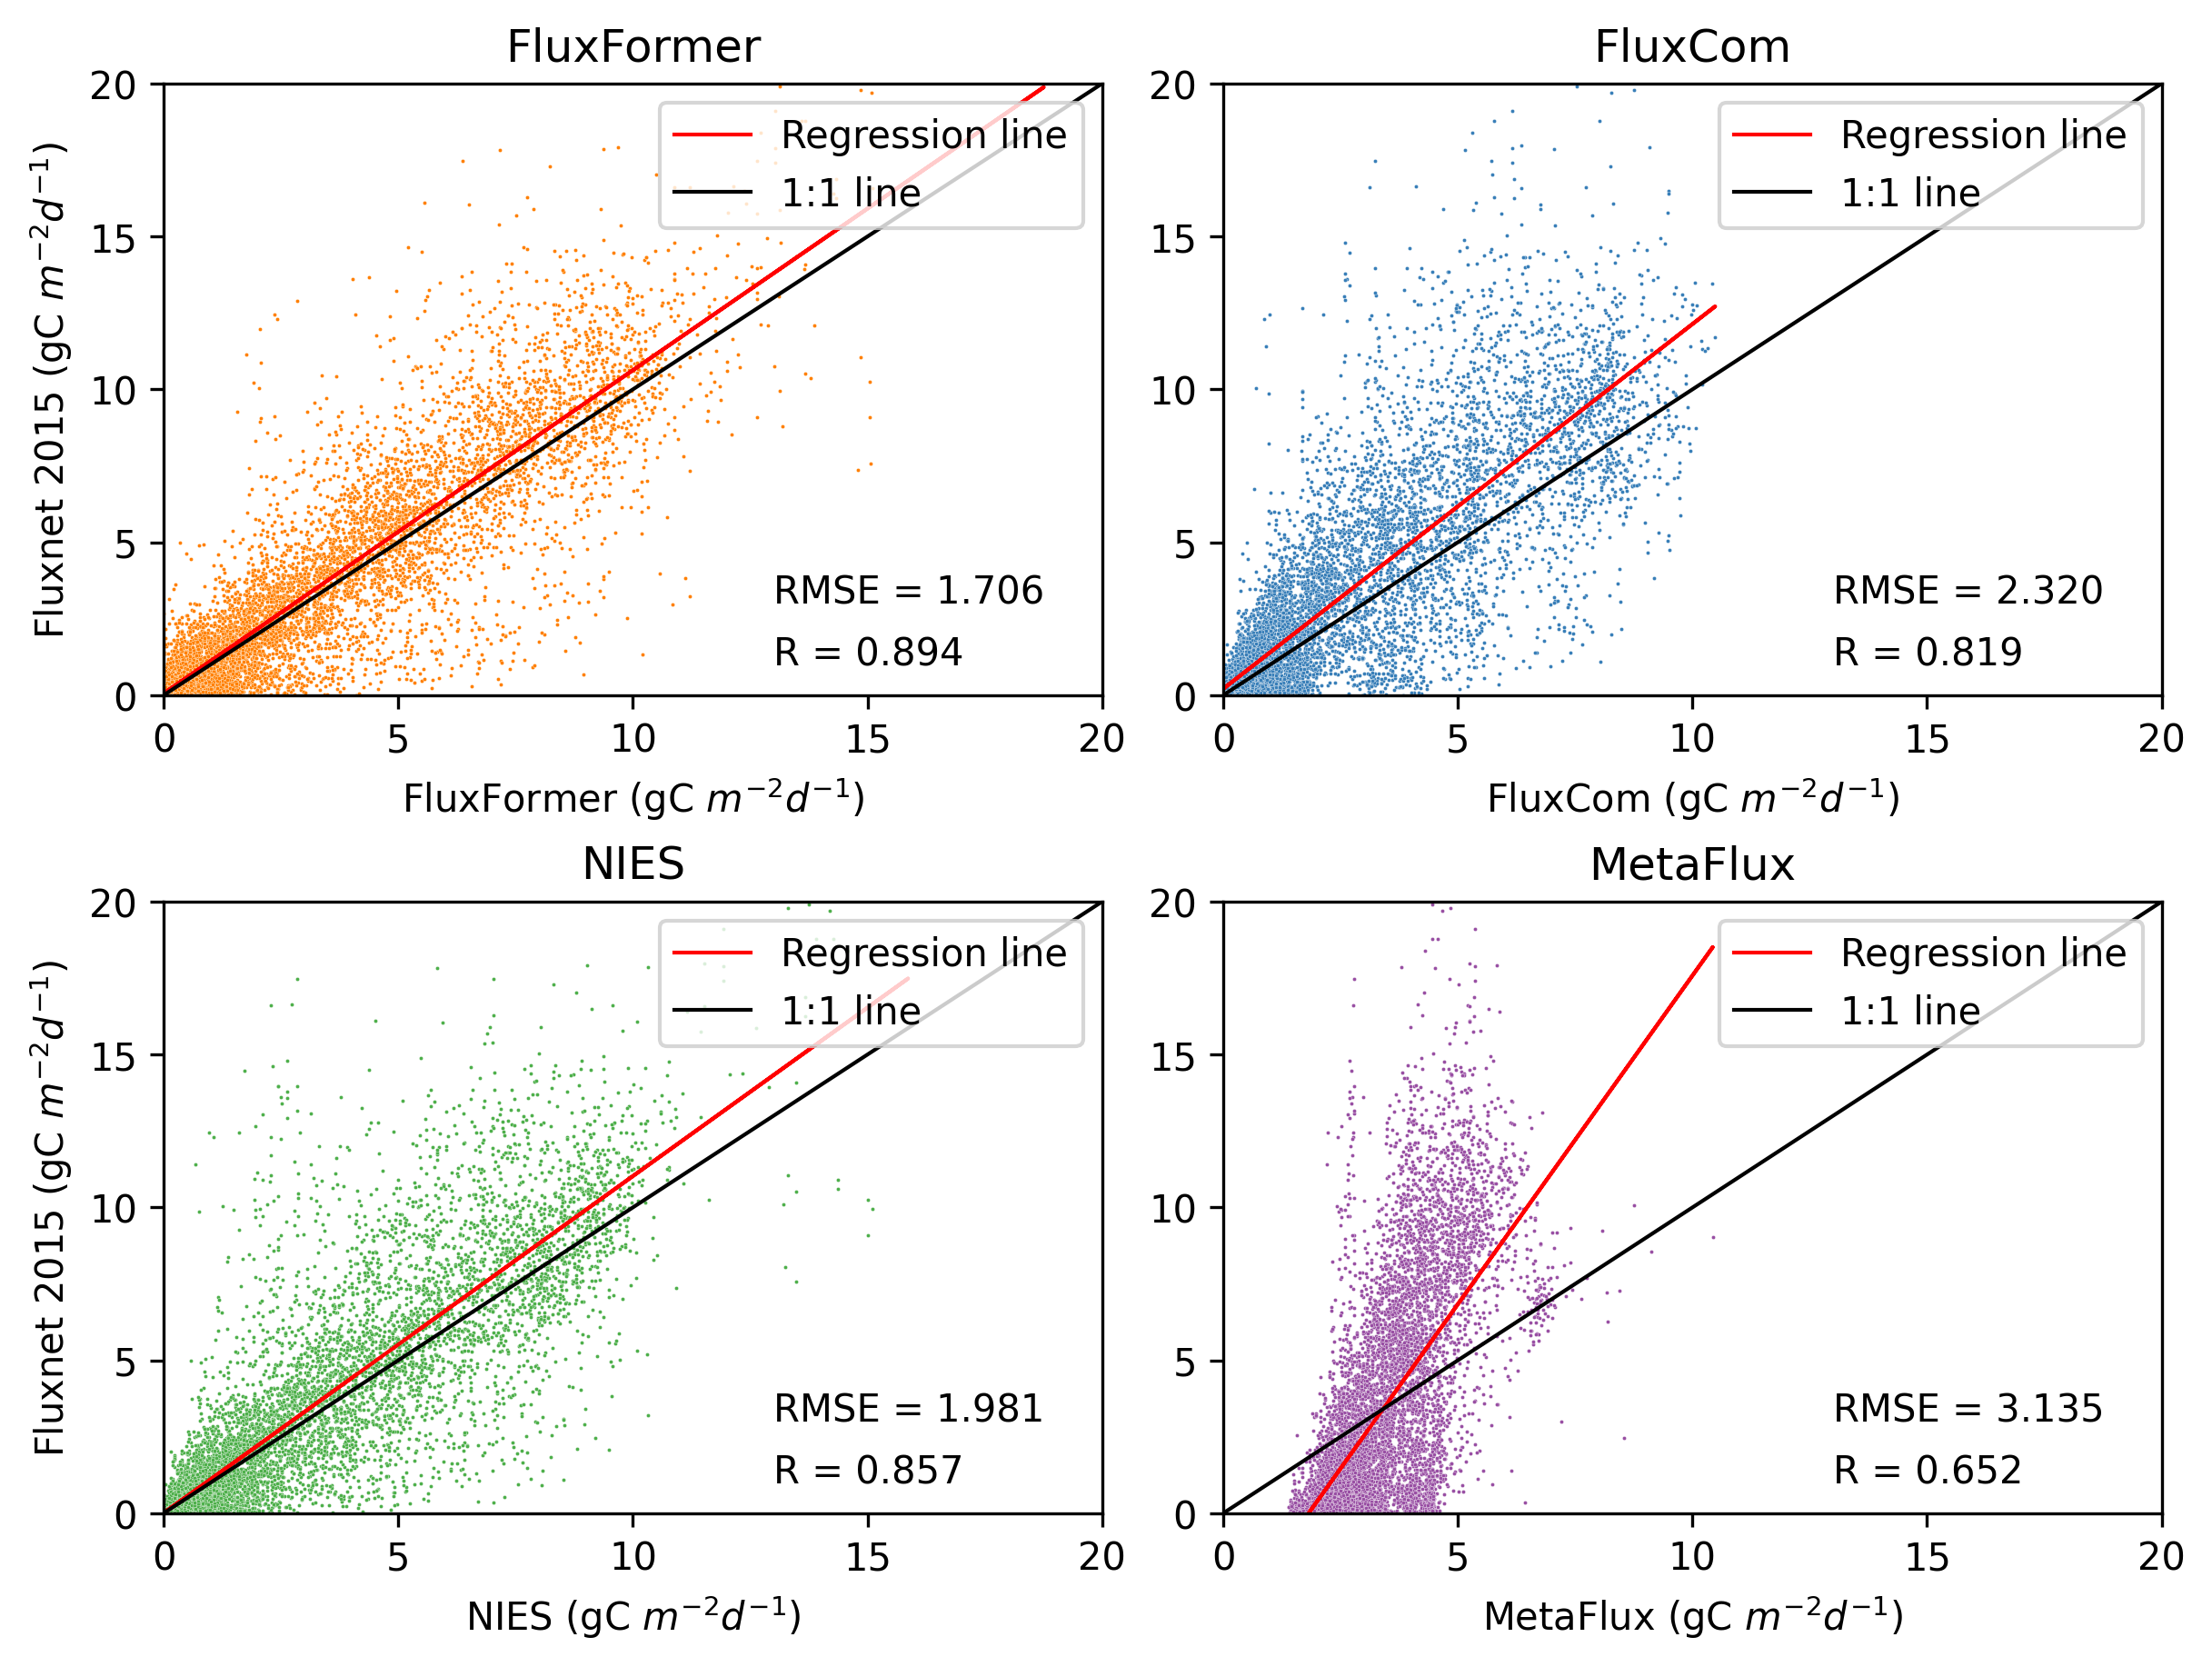
\includegraphics[width=.8\textwidth]{figs/chap6/val_fluxnet_all_GPP.png}
      \caption{GPP}
      \label{fig:chap6_fig3a}
    \end{subfigure}

    \begin{subfigure}{\textwidth}
      \centering
      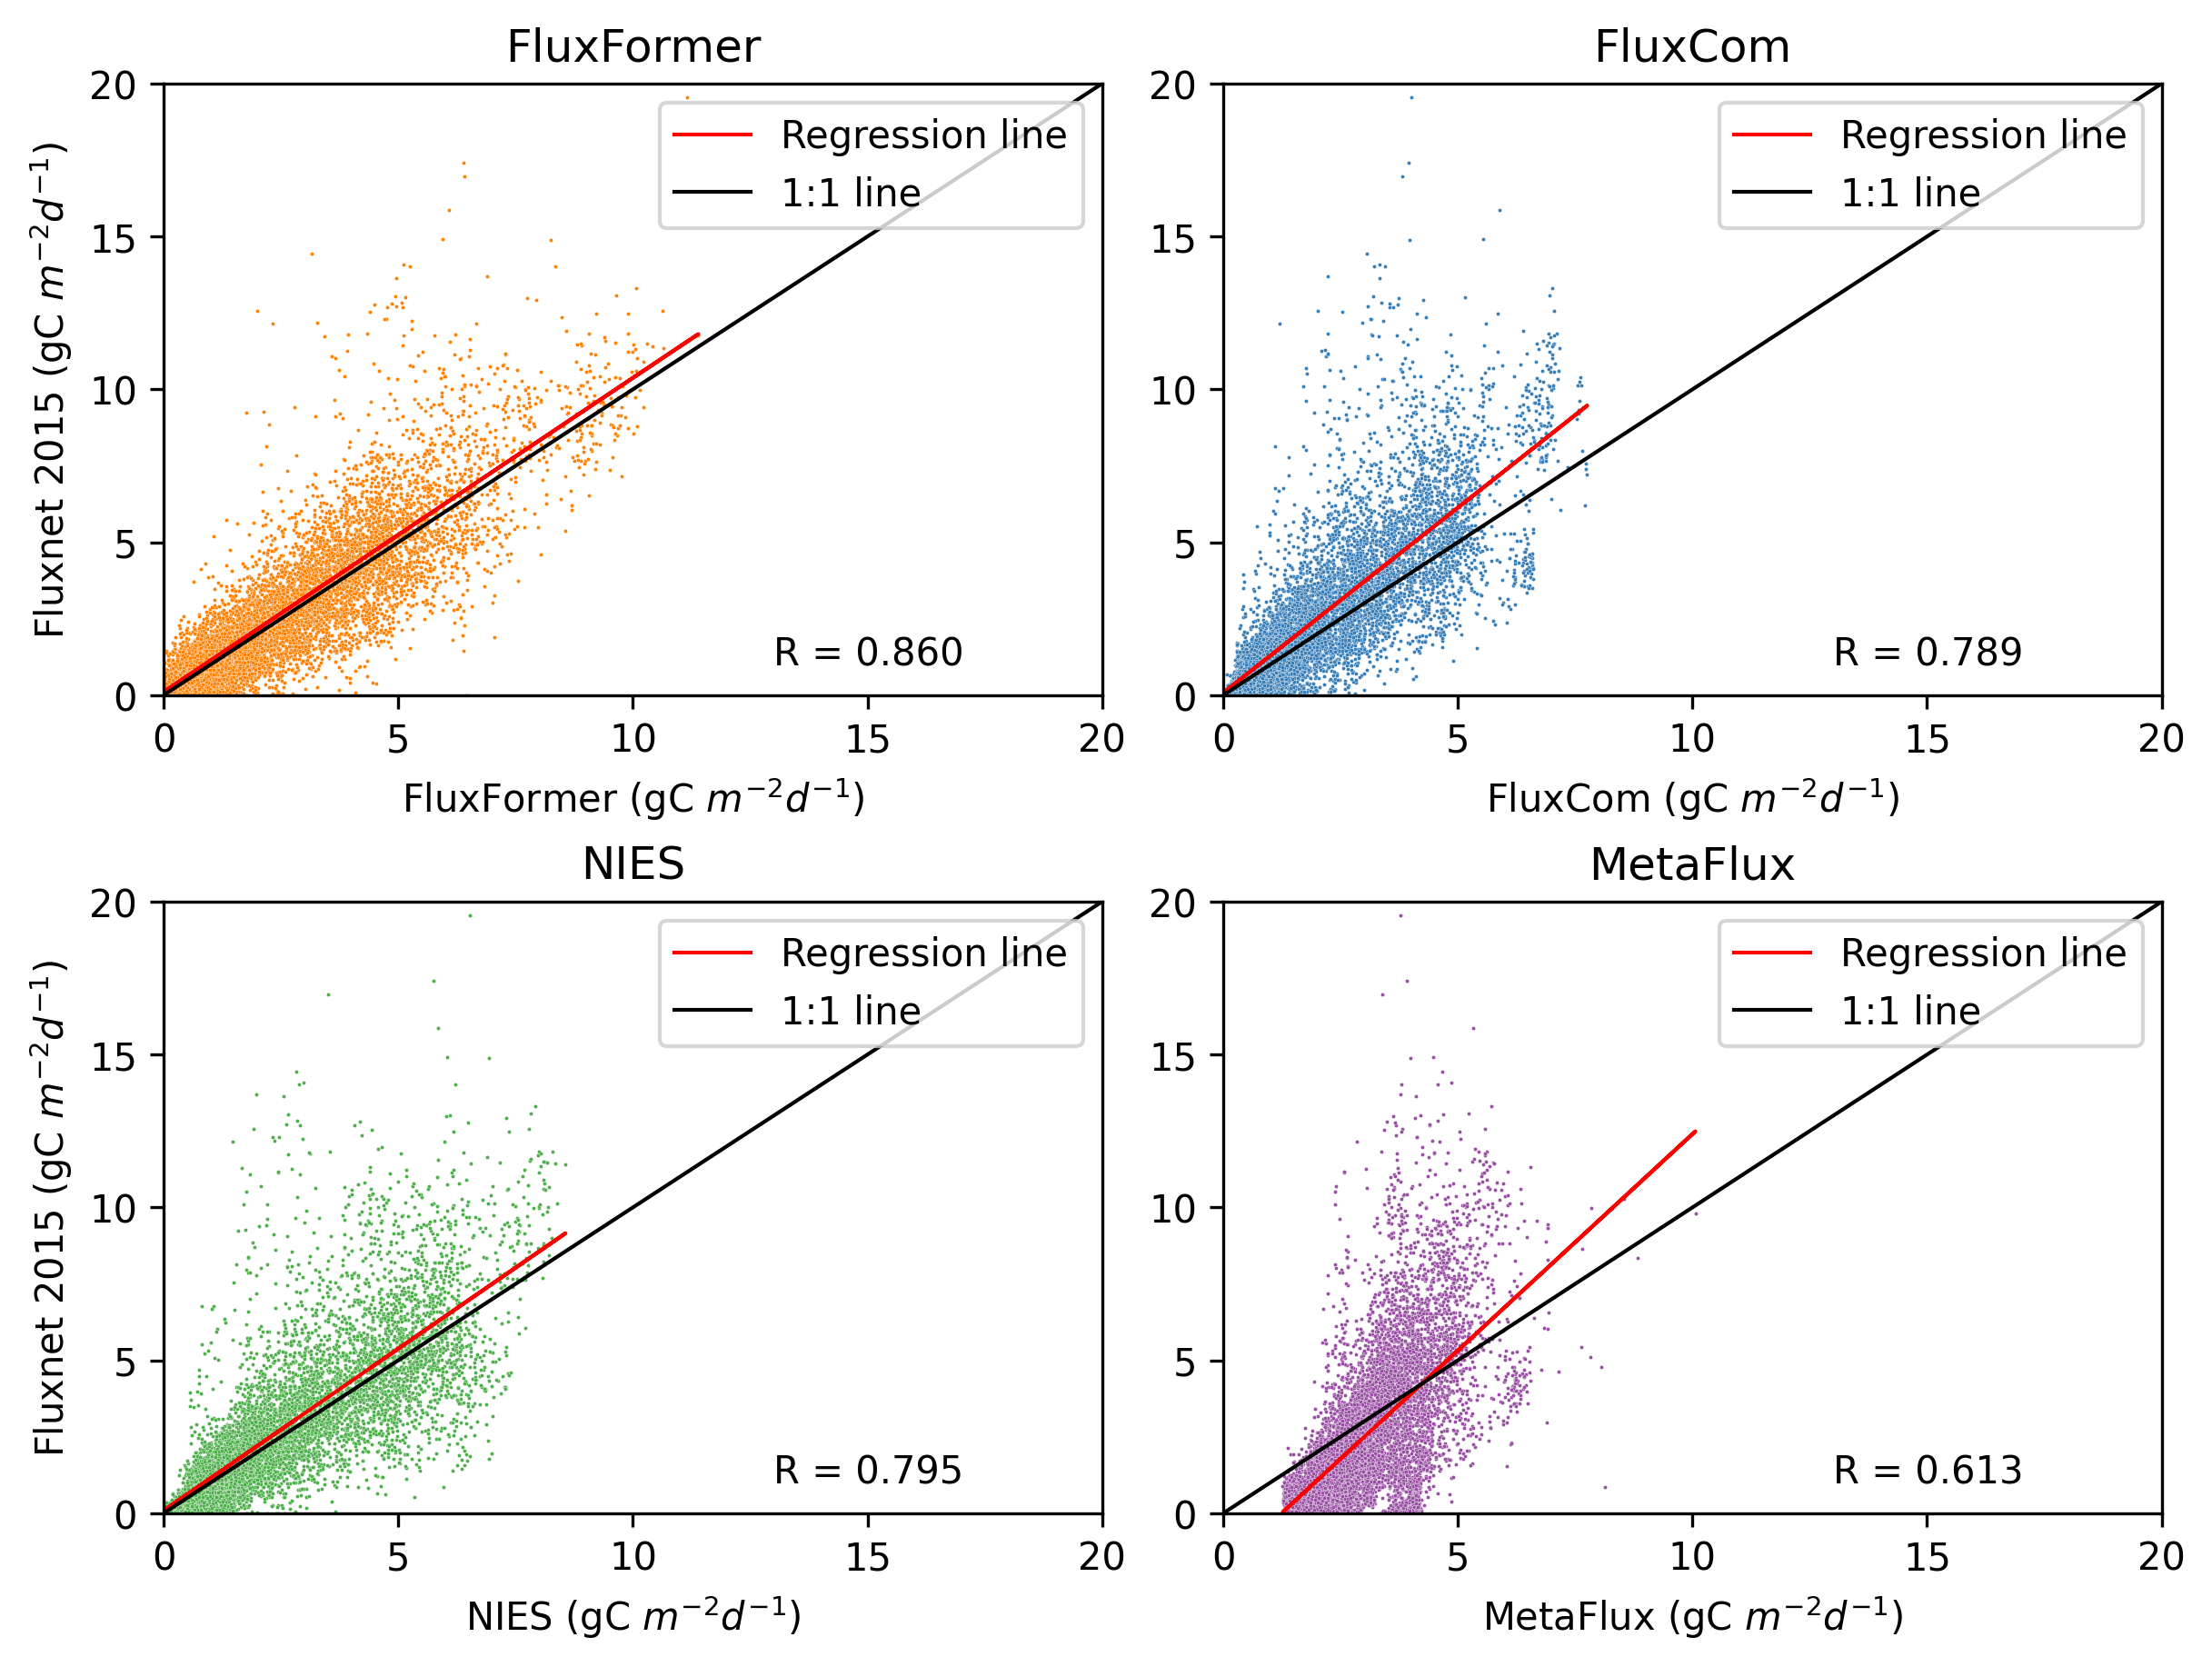
\includegraphics[width=.8\textwidth]{figs/chap6/val_fluxnet_all_RECO.png}
      \caption{RECO}
      \label{fig:chap6_fig3b}
    \end{subfigure}
    \caption[Validation with FLUXNET 2015]{Validation with FLUXNET 2015: GPP (a) RECO (b)}
    \label{fig:chap6_fig3}
\end{figure}
\subsubsection*{Seasonality validation}
We also examined the seasonal trend with the FLUXNET 2015 data. We calculate the monthly mean fluxes for 
\begin{figure}[p]
    \centering
    \begin{subfigure}{\textwidth}
      \centering
      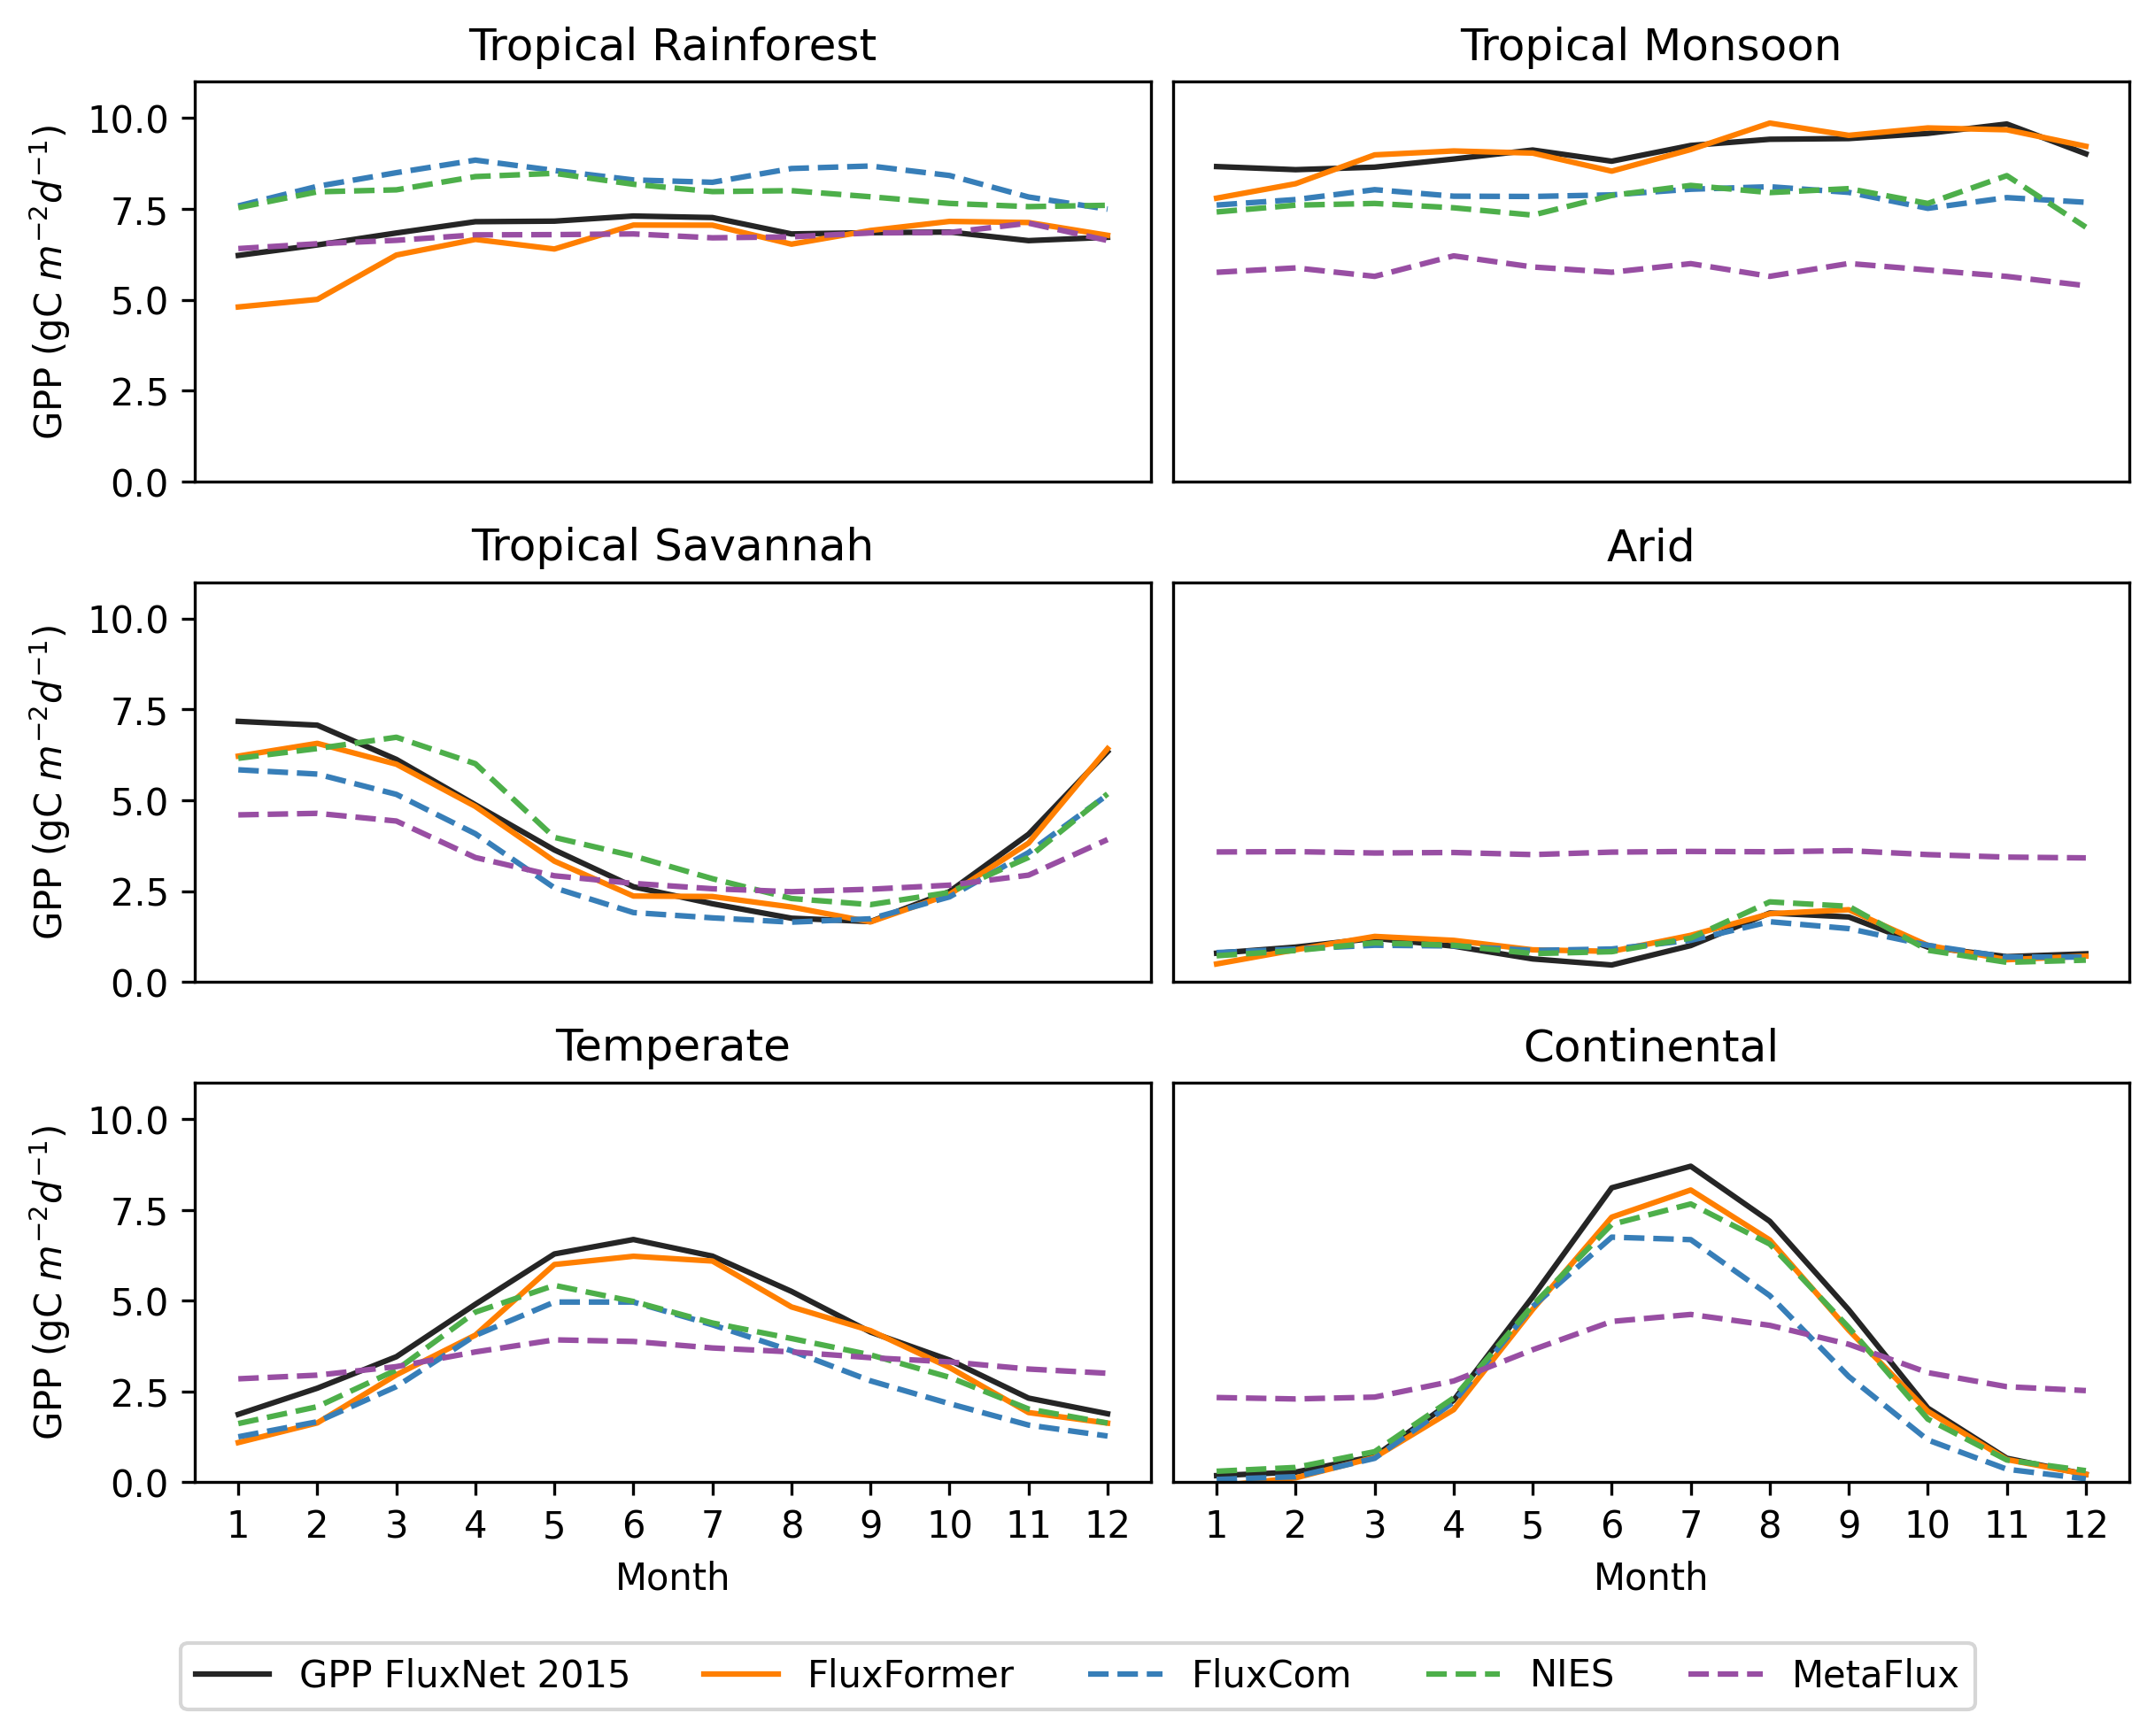
\includegraphics[width=.8\textwidth]{figs/chap6/seasonal_fluxnet_GPP.png}
      \caption{GPP}
      \label{fig:chap6_fig4a}
    \end{subfigure}

    \begin{subfigure}{\textwidth}
      \centering
      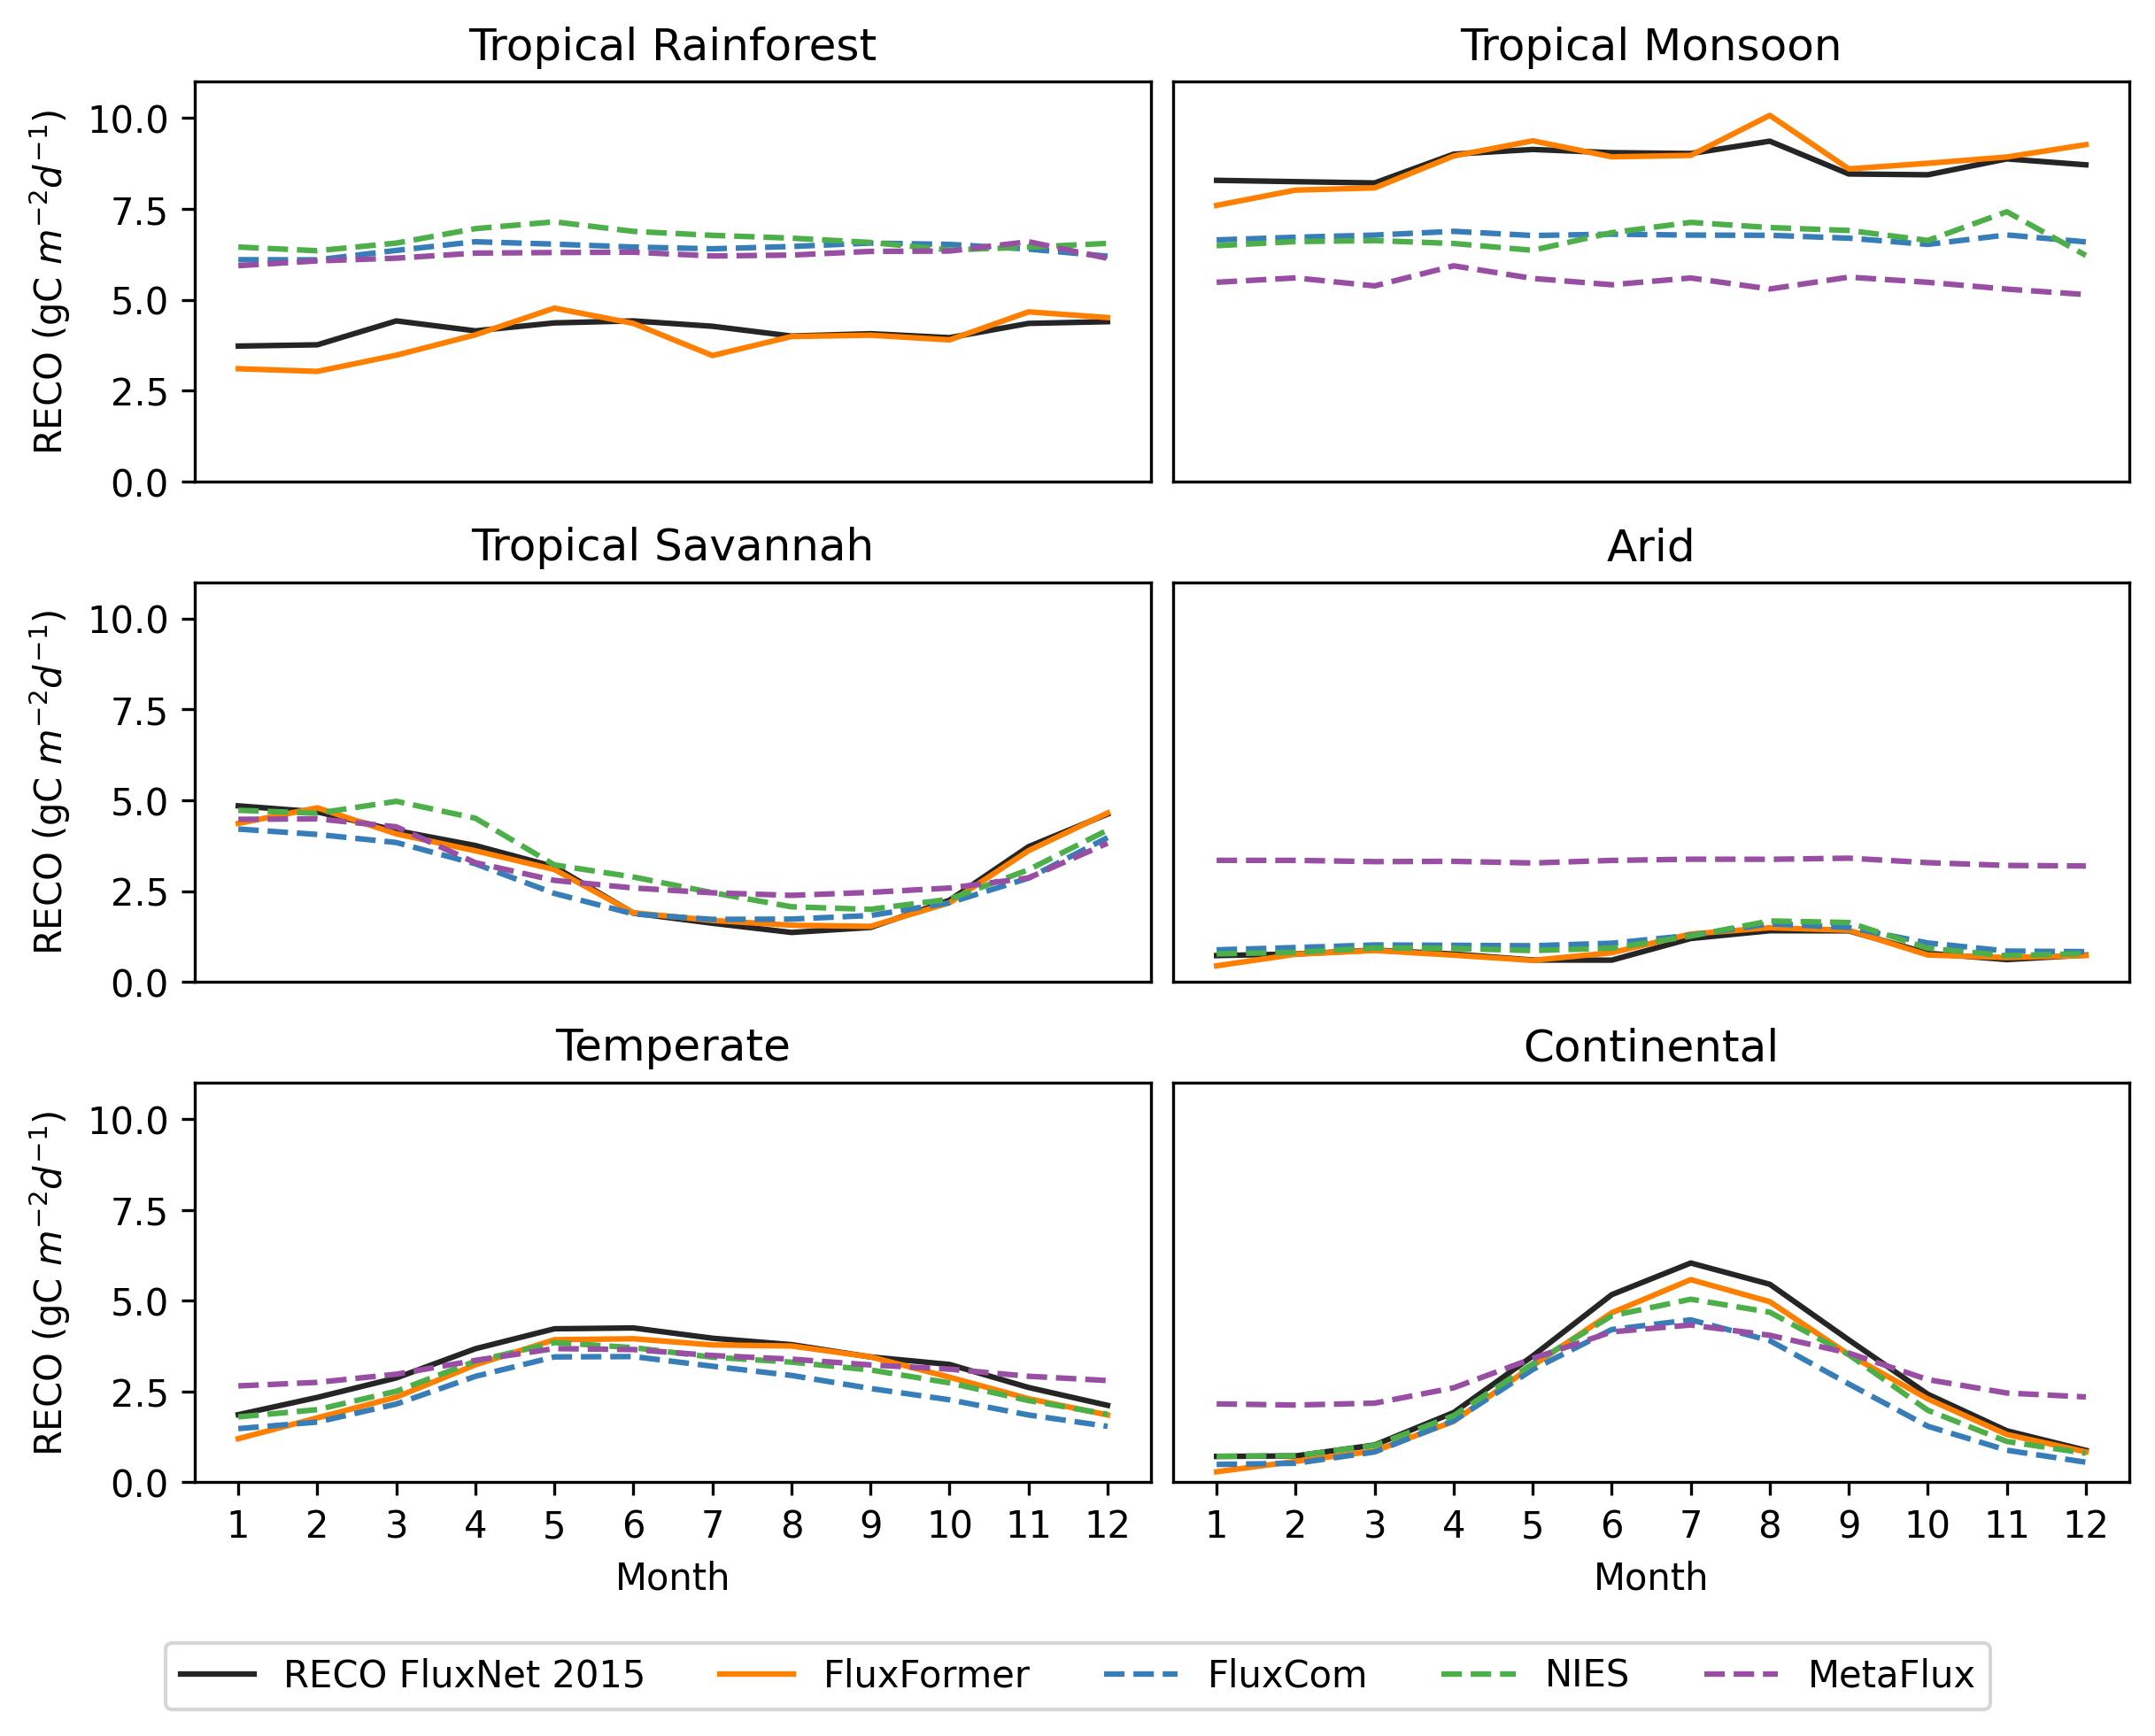
\includegraphics[width=.8\textwidth]{figs/chap6/seasonal_fluxnet_RECO.png}
      \caption{RECO}
      \label{fig:chap6_fig4b}
    \end{subfigure}
    \caption[Seasonality validation with FLUXNET 2015]{Seasonality validation with FLUXNET 2015: GPP (a) RECO (b)}
    \label{fig:chap6_fig4}
\end{figure}

\subsection{Validation with SIF}

\begin{figure}[p]
    \centering
    \begin{subfigure}{\textwidth}
      \centering
      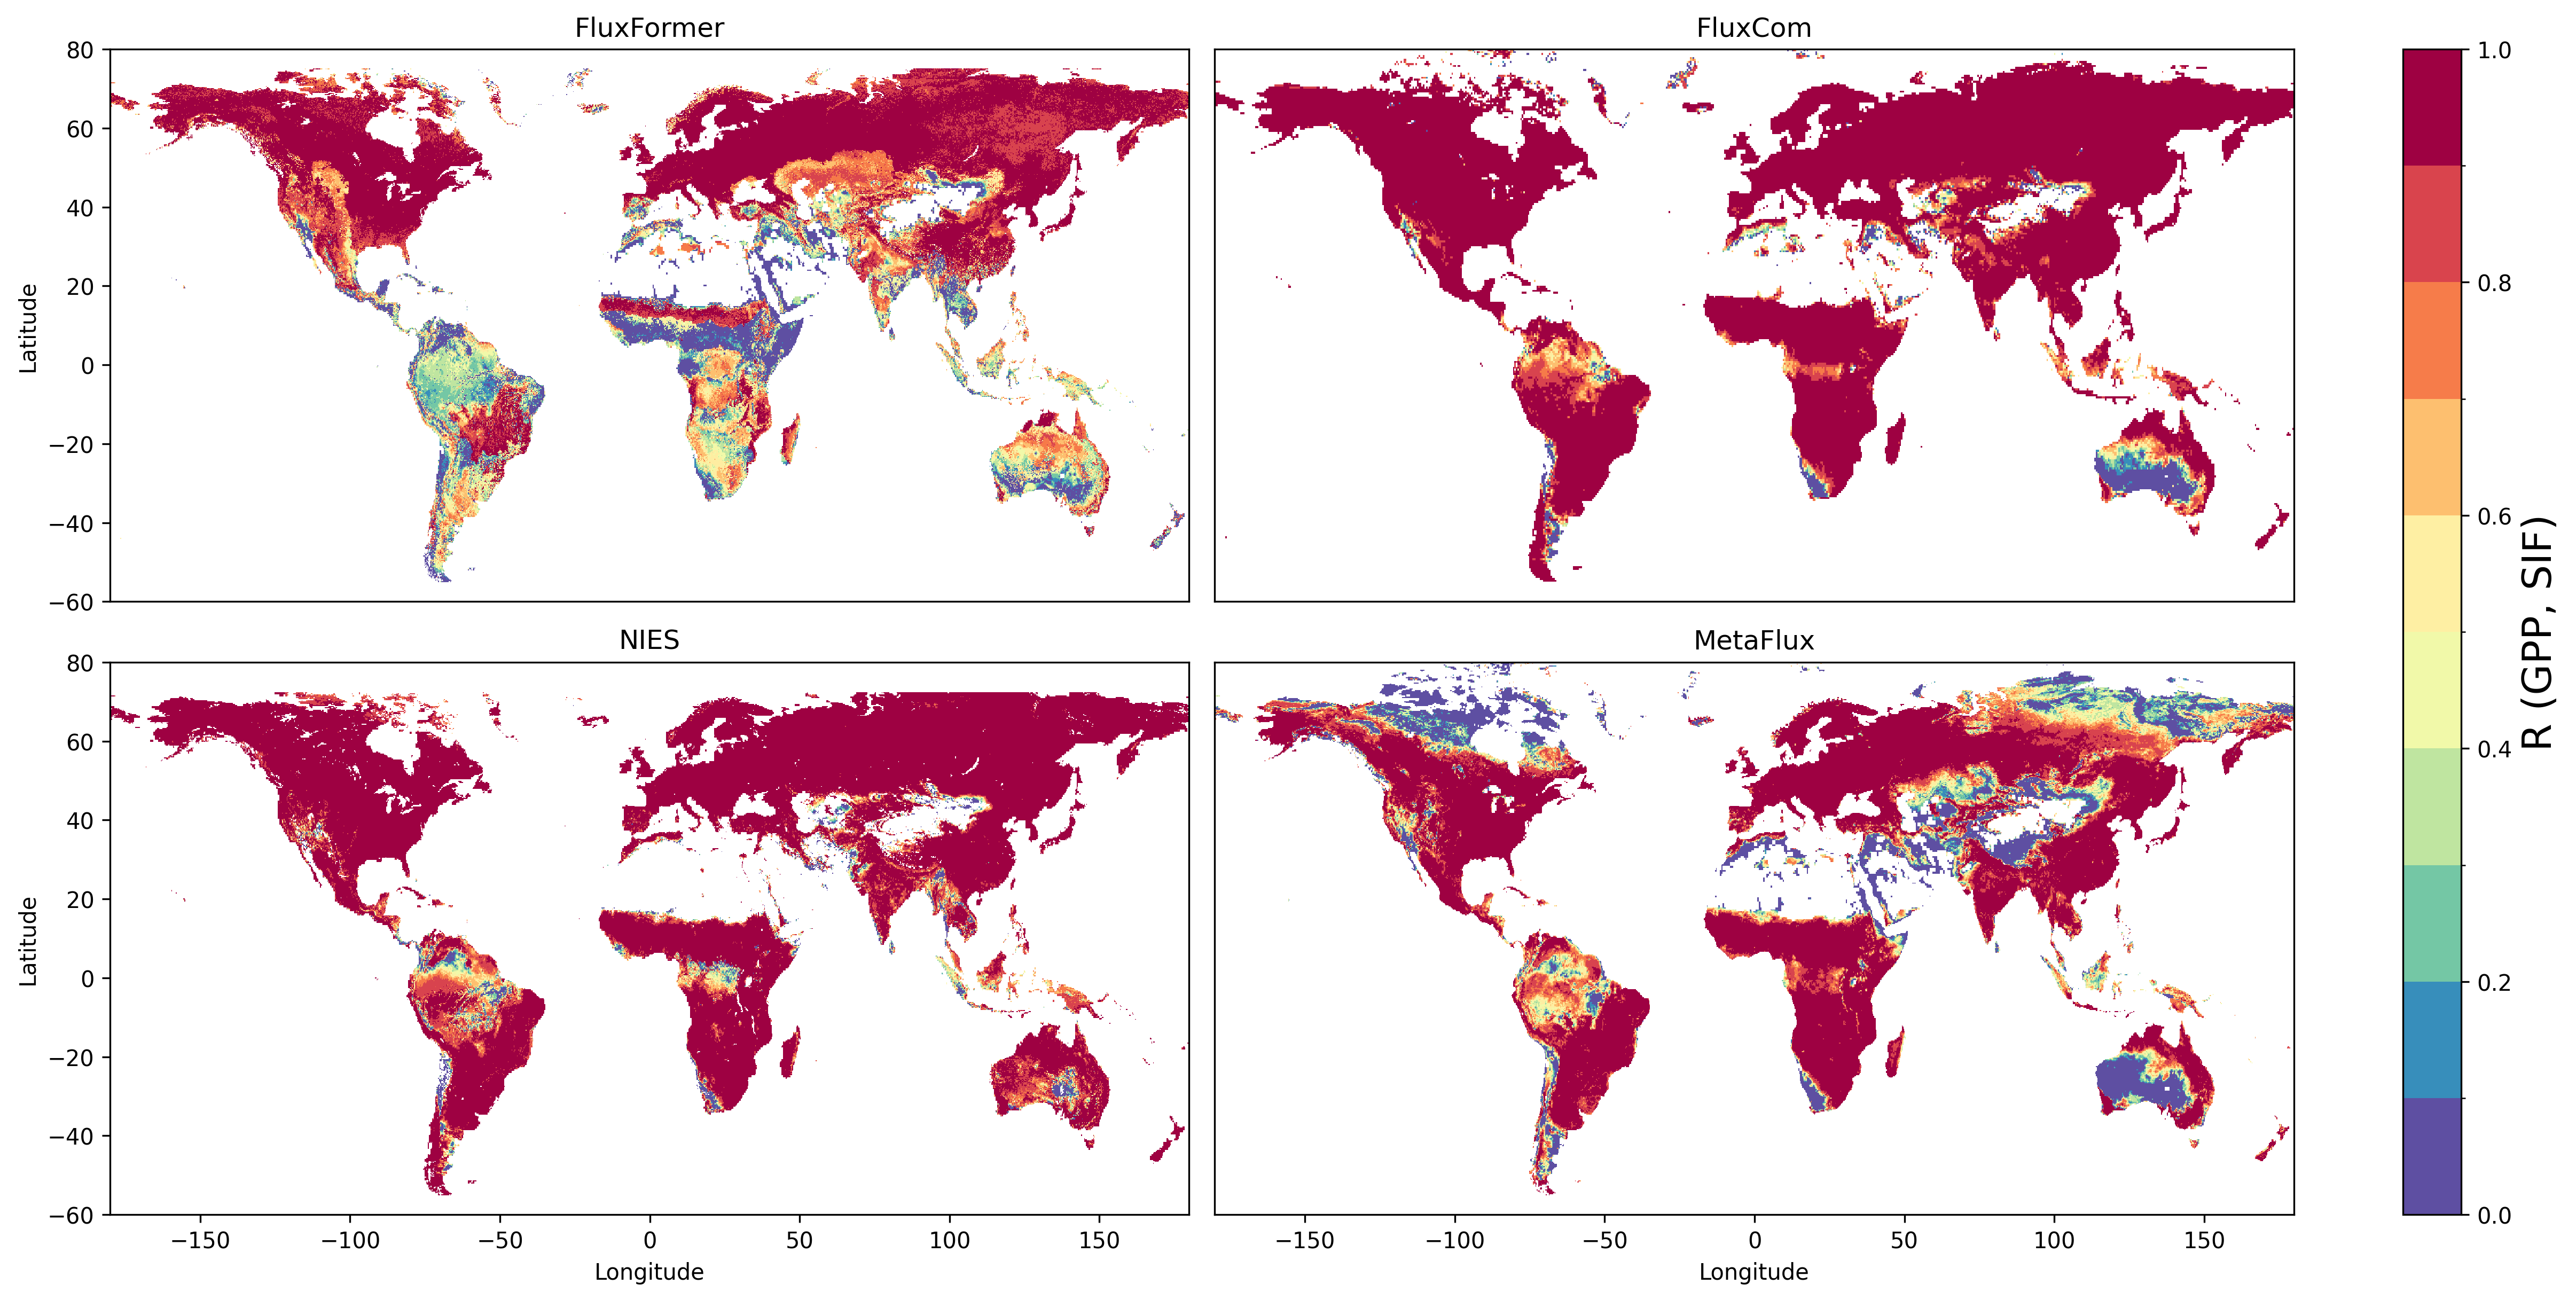
\includegraphics[width=\textwidth]{figs/chap6/val_CSIF.png}
      \caption{CSIF}
      \label{fig:chap6_fig5a}
    \end{subfigure}

    \begin{subfigure}{\textwidth}
      \centering
      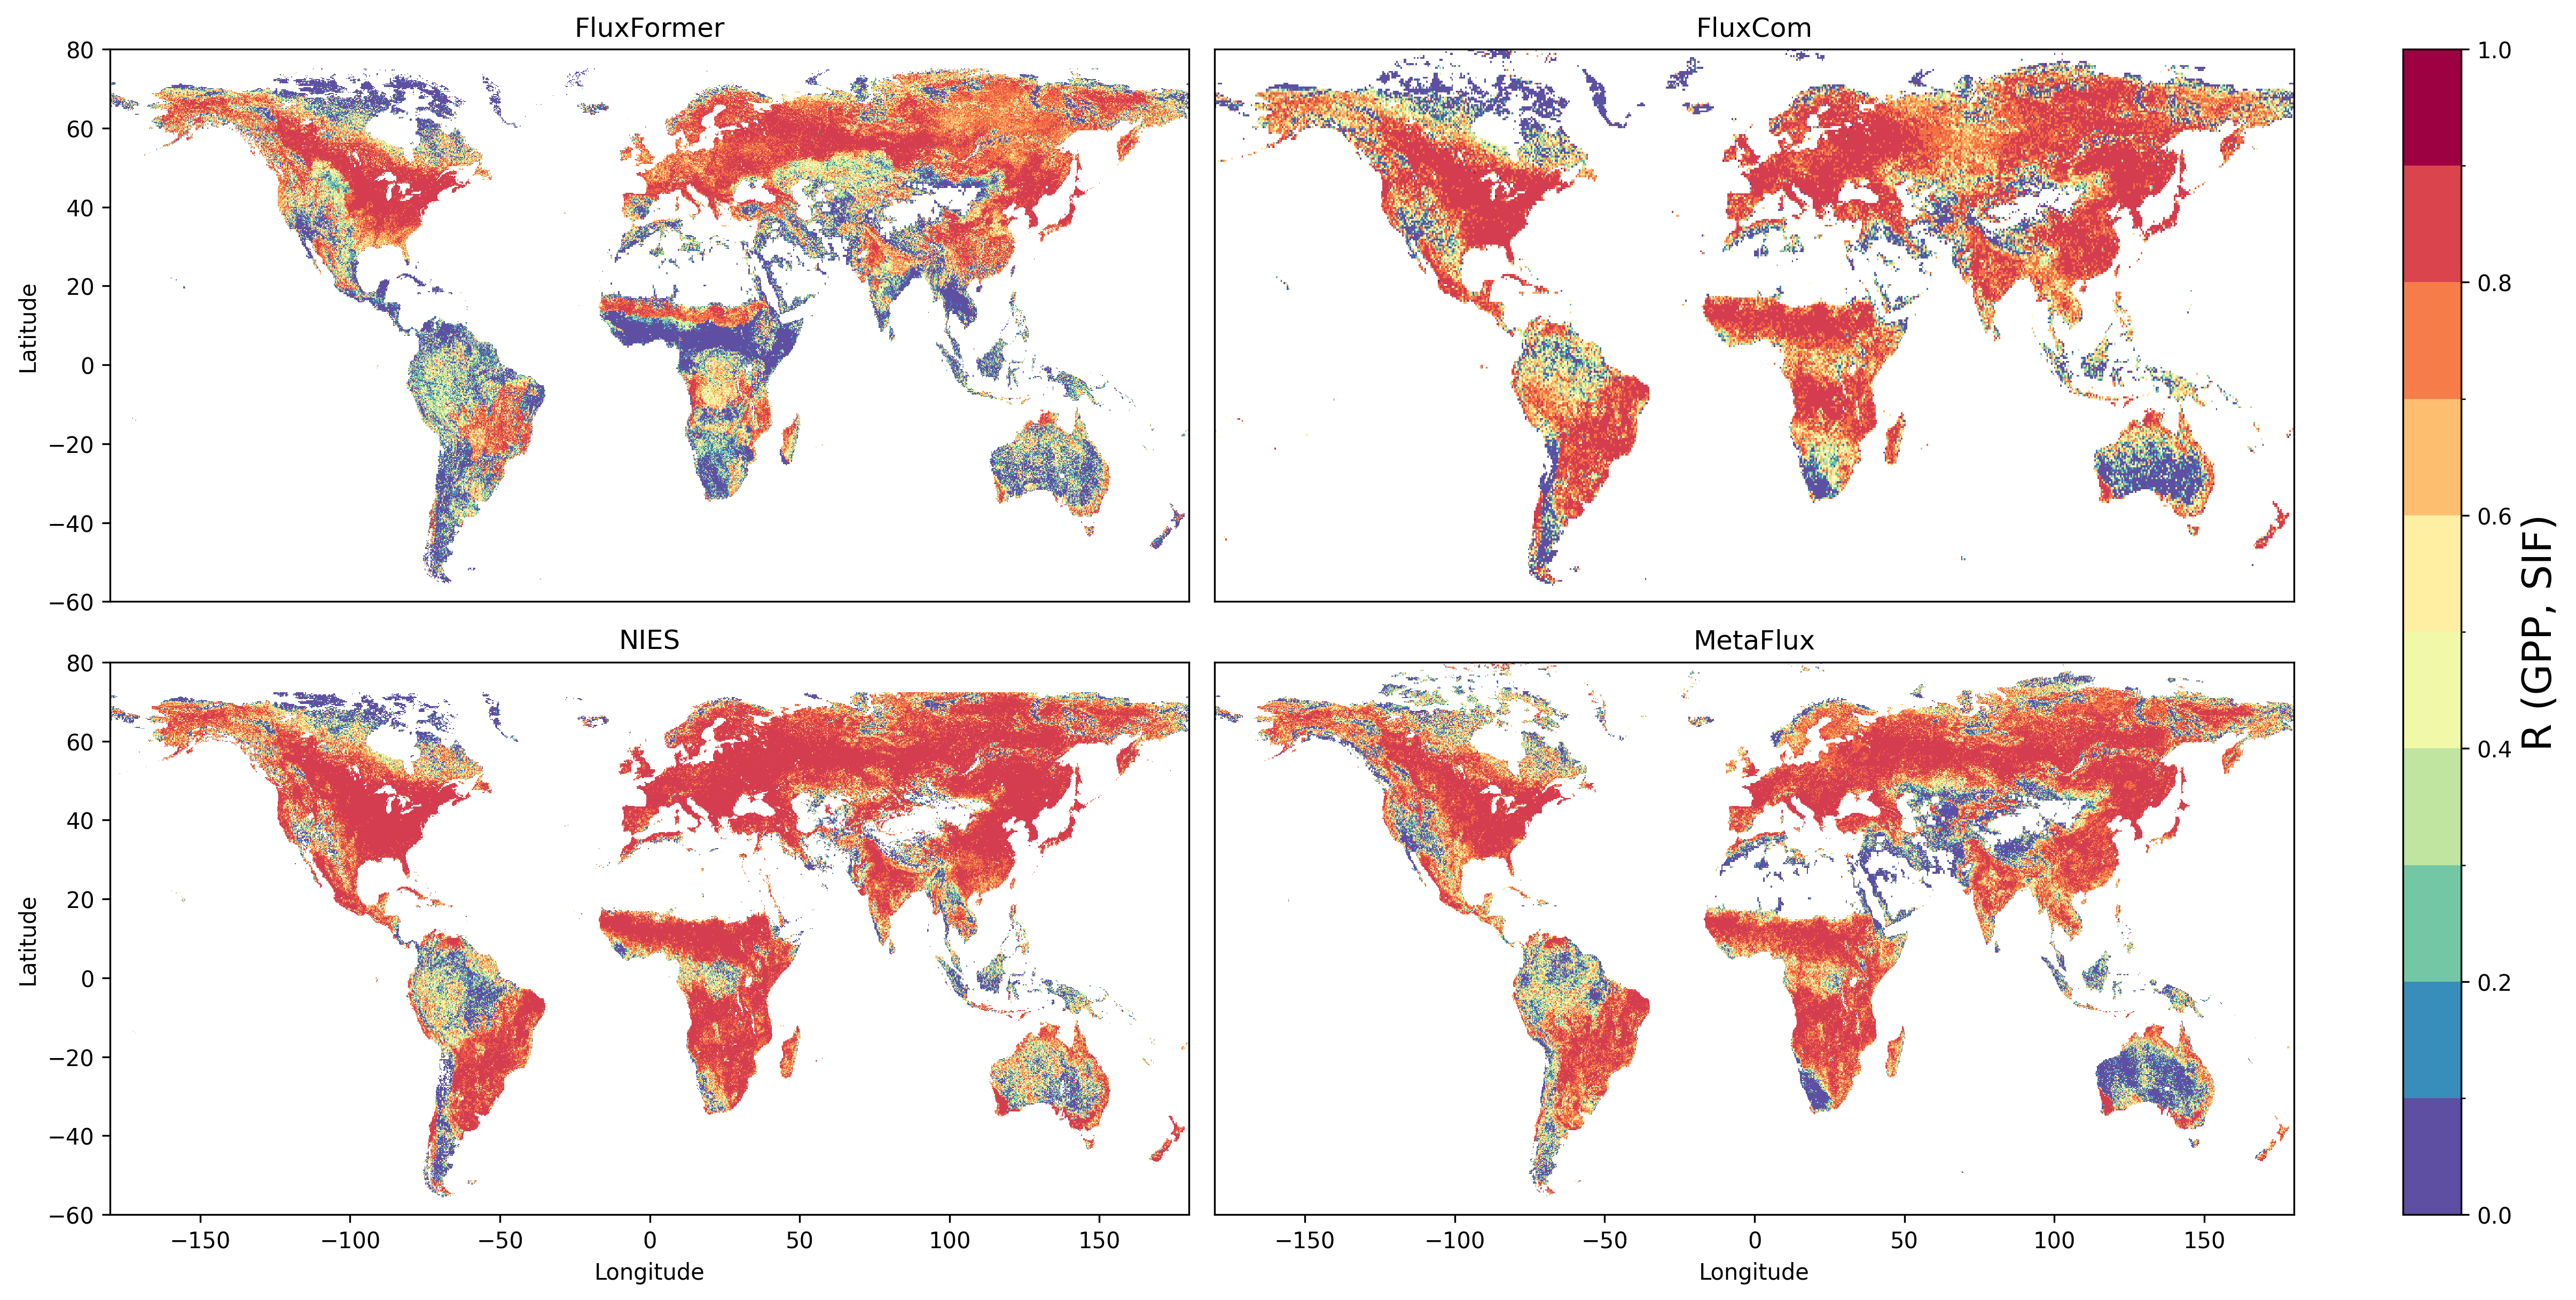
\includegraphics[width=\textwidth]{figs/chap6/val_TROPOMI_SIF.png}
      \caption{TROPOMI SIF}
      \label{fig:chap6_fig5b}
    \end{subfigure}
    \caption[Validation with SIF products]{Validation with SIF products: CSIF (a) TROPOMI SIF (b)}
    \label{fig:chap6_fig5}
\end{figure}


\subsubsection*{Validation with other satellite-based products}

\begin{figure}[p]
    \centering
    \begin{subfigure}{\textwidth}
      \centering
      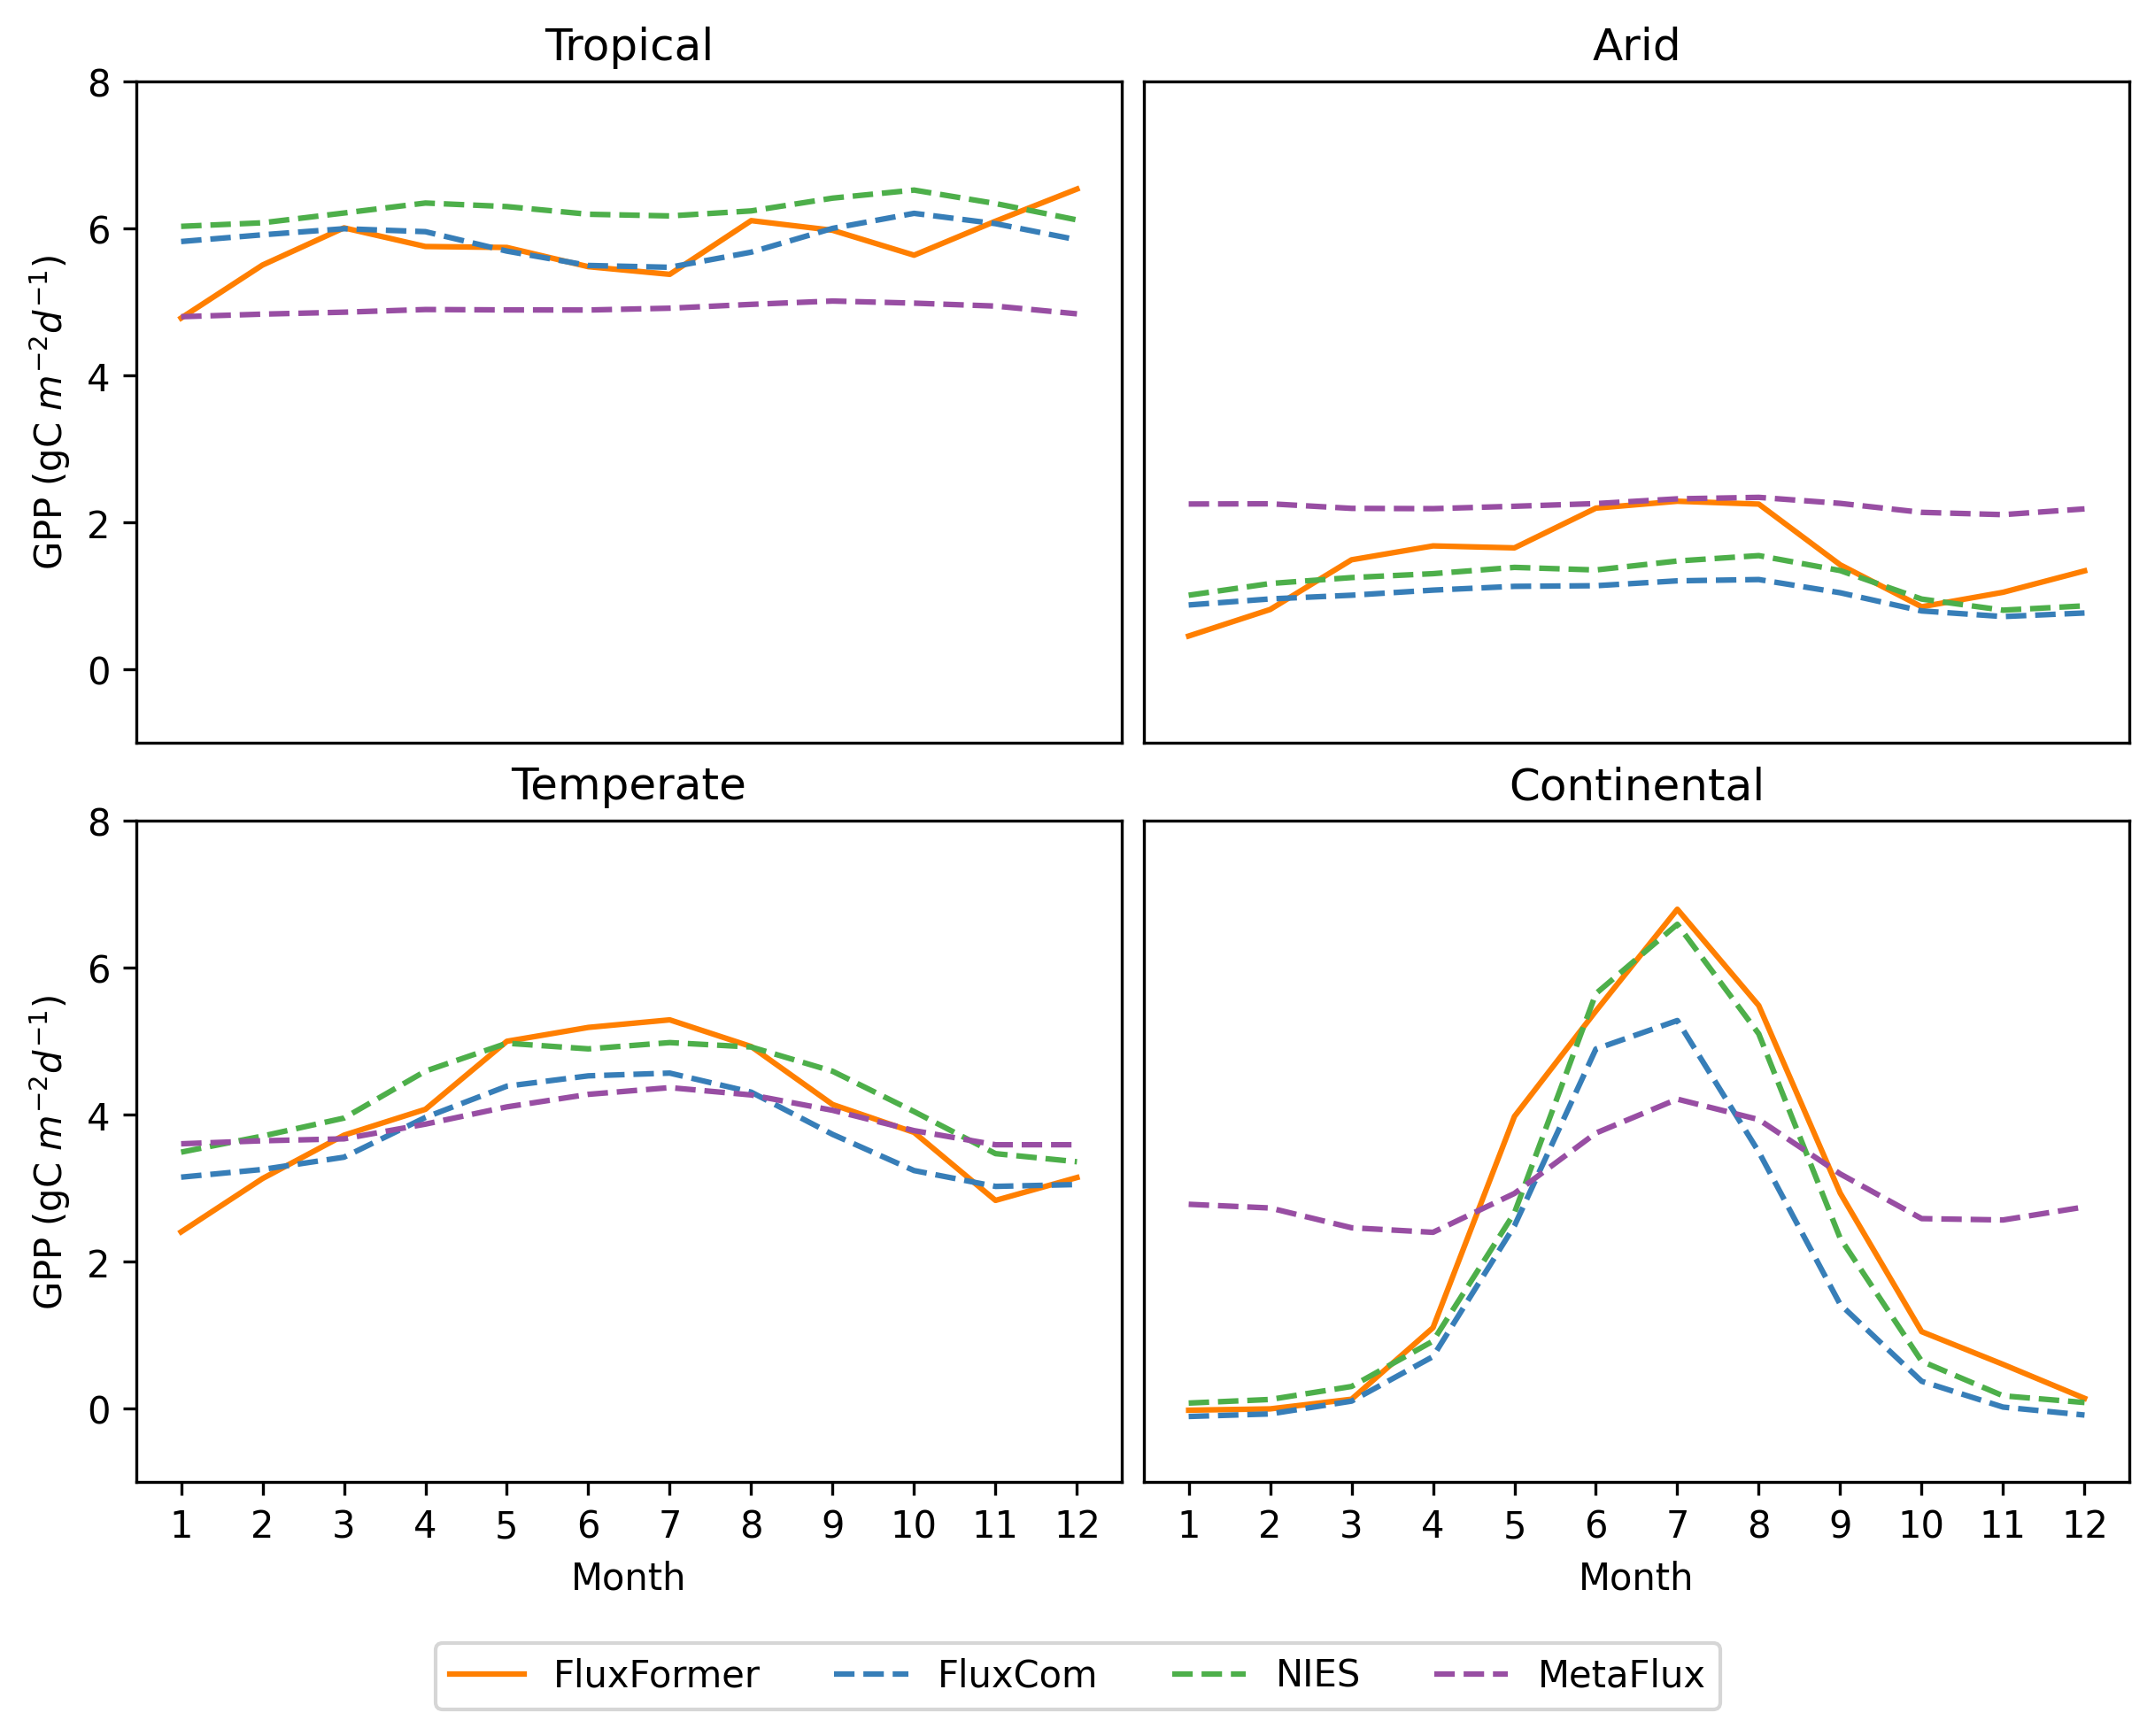
\includegraphics[width=.8\textwidth]{figs/chap6/seasonal_inter_prods_GPP.png}
      \caption{GPP}
      \label{fig:chap6_fig6a}
    \end{subfigure}

    \begin{subfigure}{\textwidth}
      \centering
      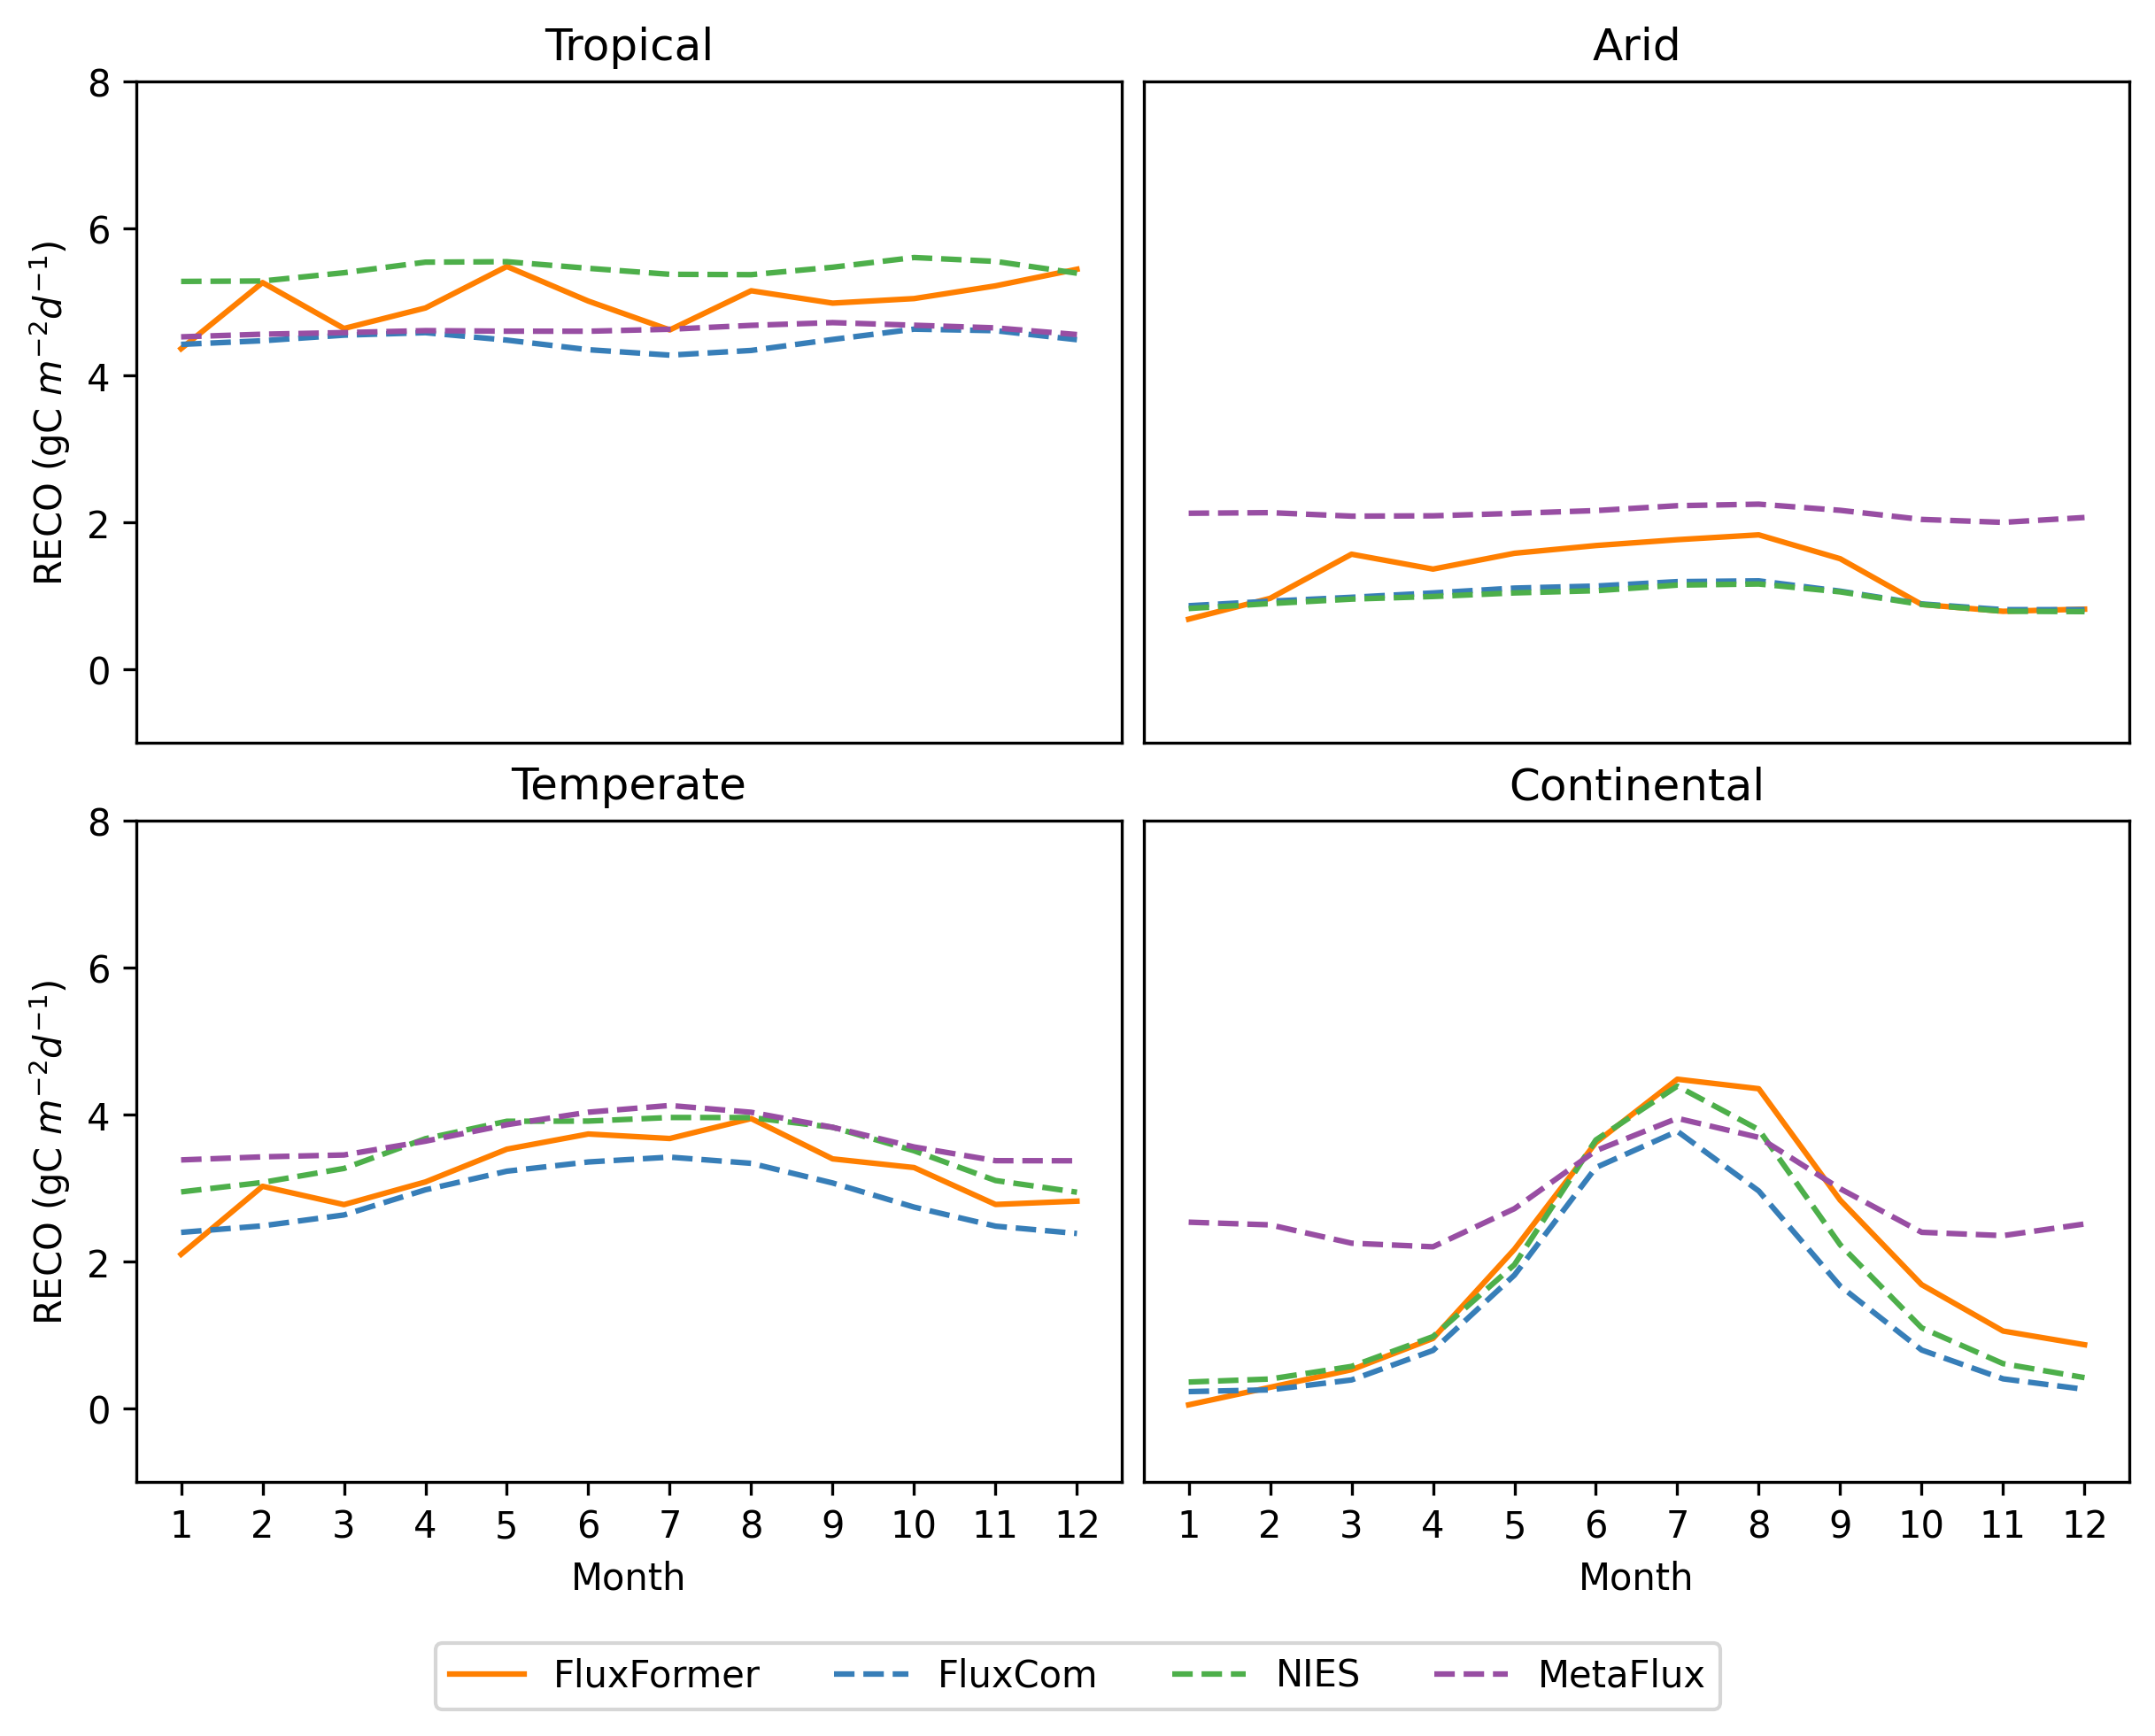
\includegraphics[width=.8\textwidth]{figs/chap6/seasonal_inter_prods_RECO.png}
      \caption{RECO}
      \label{fig:chap6_fig6b}
    \end{subfigure}
    \caption[Seasonality validation with FLUXNET 2015]{Seasonality validation with FLUXNET 2015: GPP (a) RECO (b)}
    \label{fig:chap6_fig6}
\end{figure}

\subsection{Interannual variations between products}

\begin{figure}[p]
    \centering
    \begin{subfigure}{\textwidth}
      \centering
      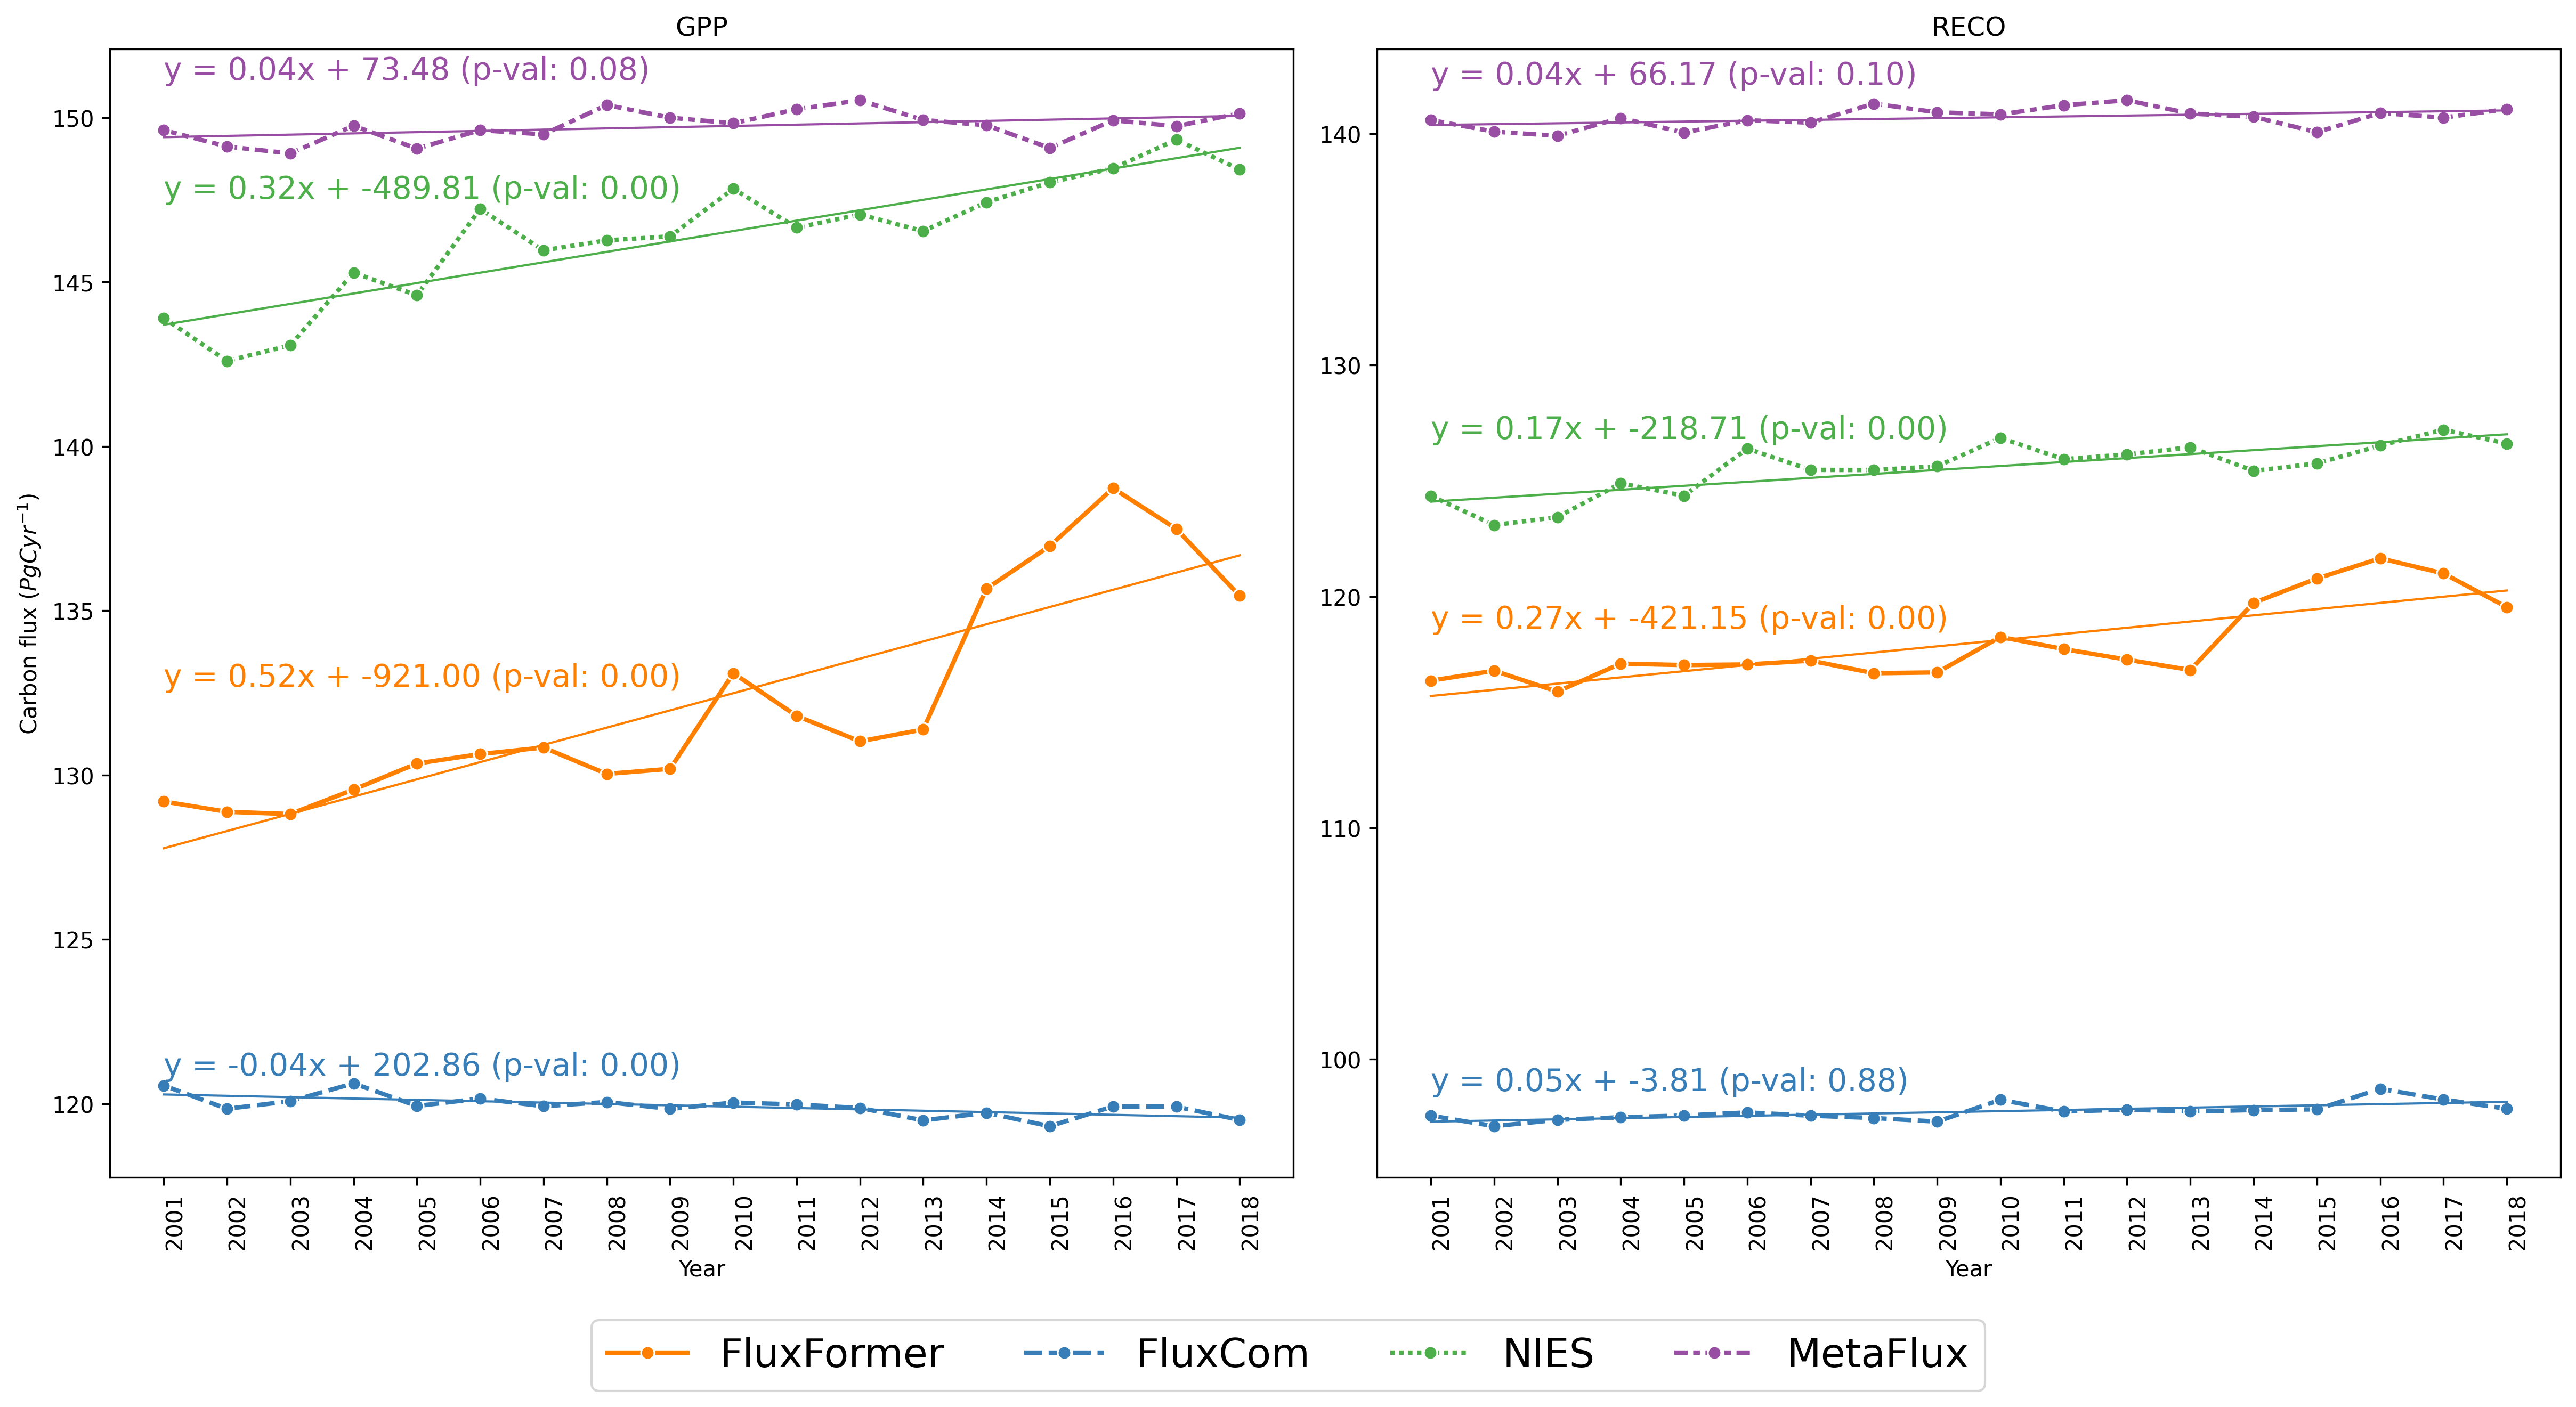
\includegraphics[width=\textwidth]{figs/chap6/global_annual_timeseries.png}
      \caption{Global annual mean timeseries from 2001 to 2019}
      \label{fig:chap6_fig7a}
    \end{subfigure}

    \begin{subfigure}{\textwidth}
      \centering
      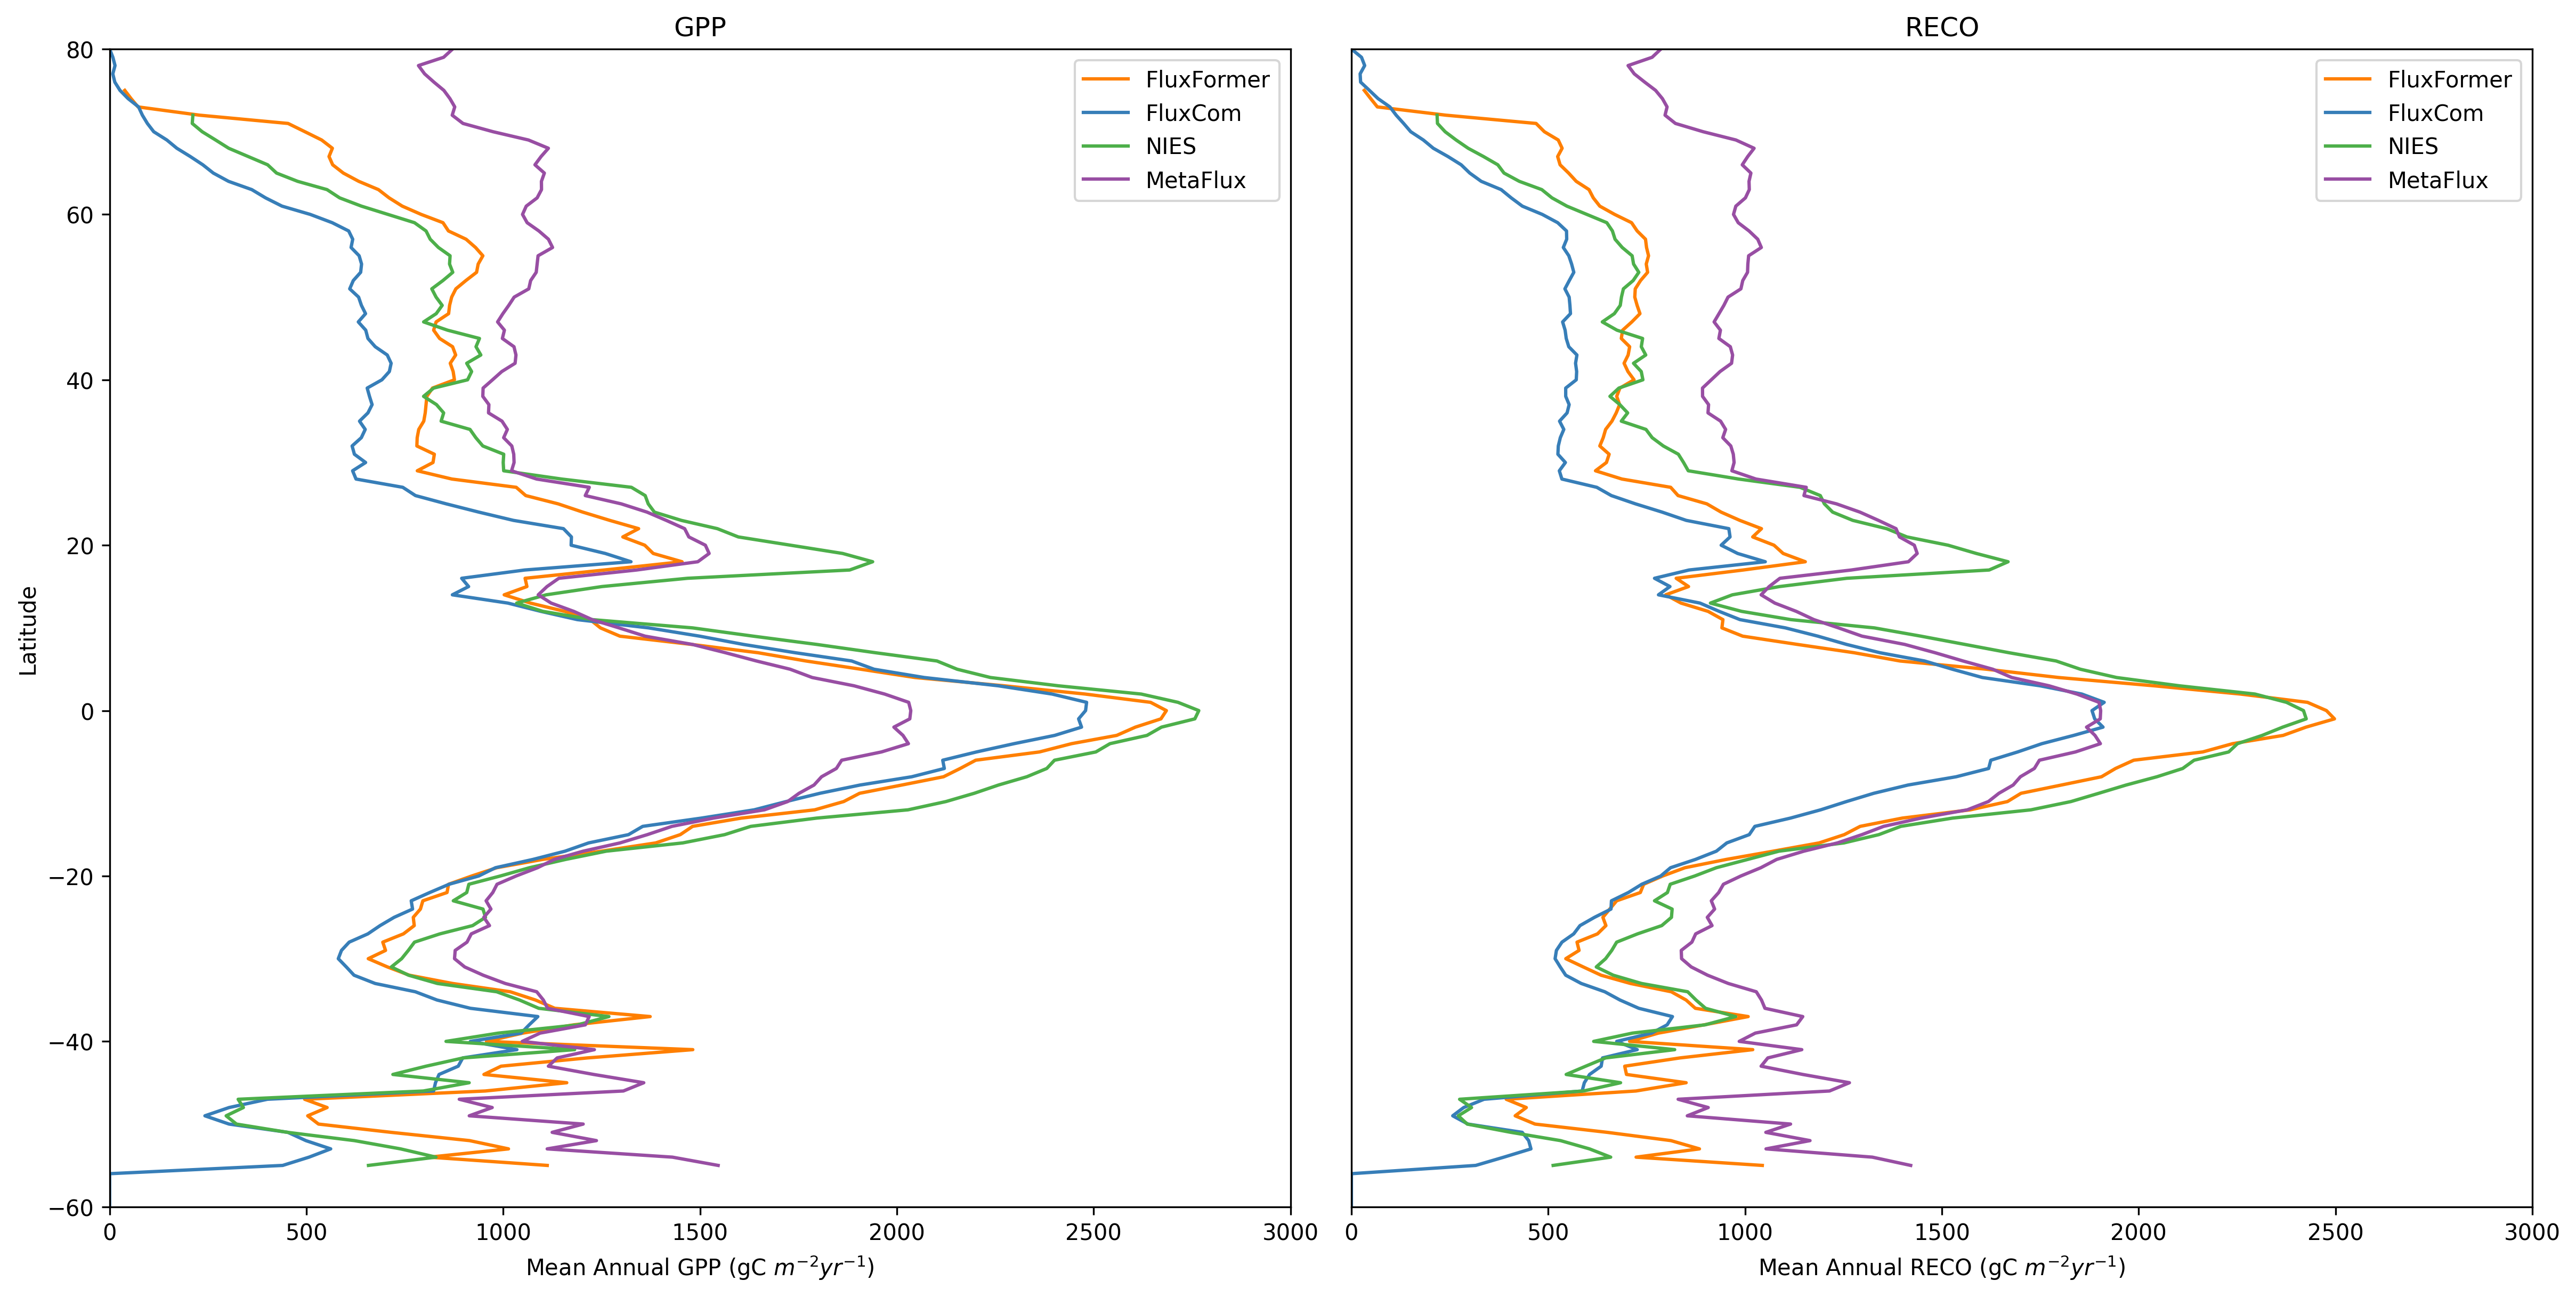
\includegraphics[width=\textwidth]{figs/chap6/lat_mean.png}
      \caption{Global annual mean distribution by latitude from 2001 to 2019}
      \label{fig:chap6_fig7b}
    \end{subfigure}
    \caption[Seasonality validation with FLUXNET 2015]{Seasonality validation with FLUXNET 2015: GPP (a) RECO (b)}
    \label{fig:chap6_fig7}
\end{figure}

\begin{figure}[p]
    \centering
    \begin{subfigure}{\textwidth}
      \centering
      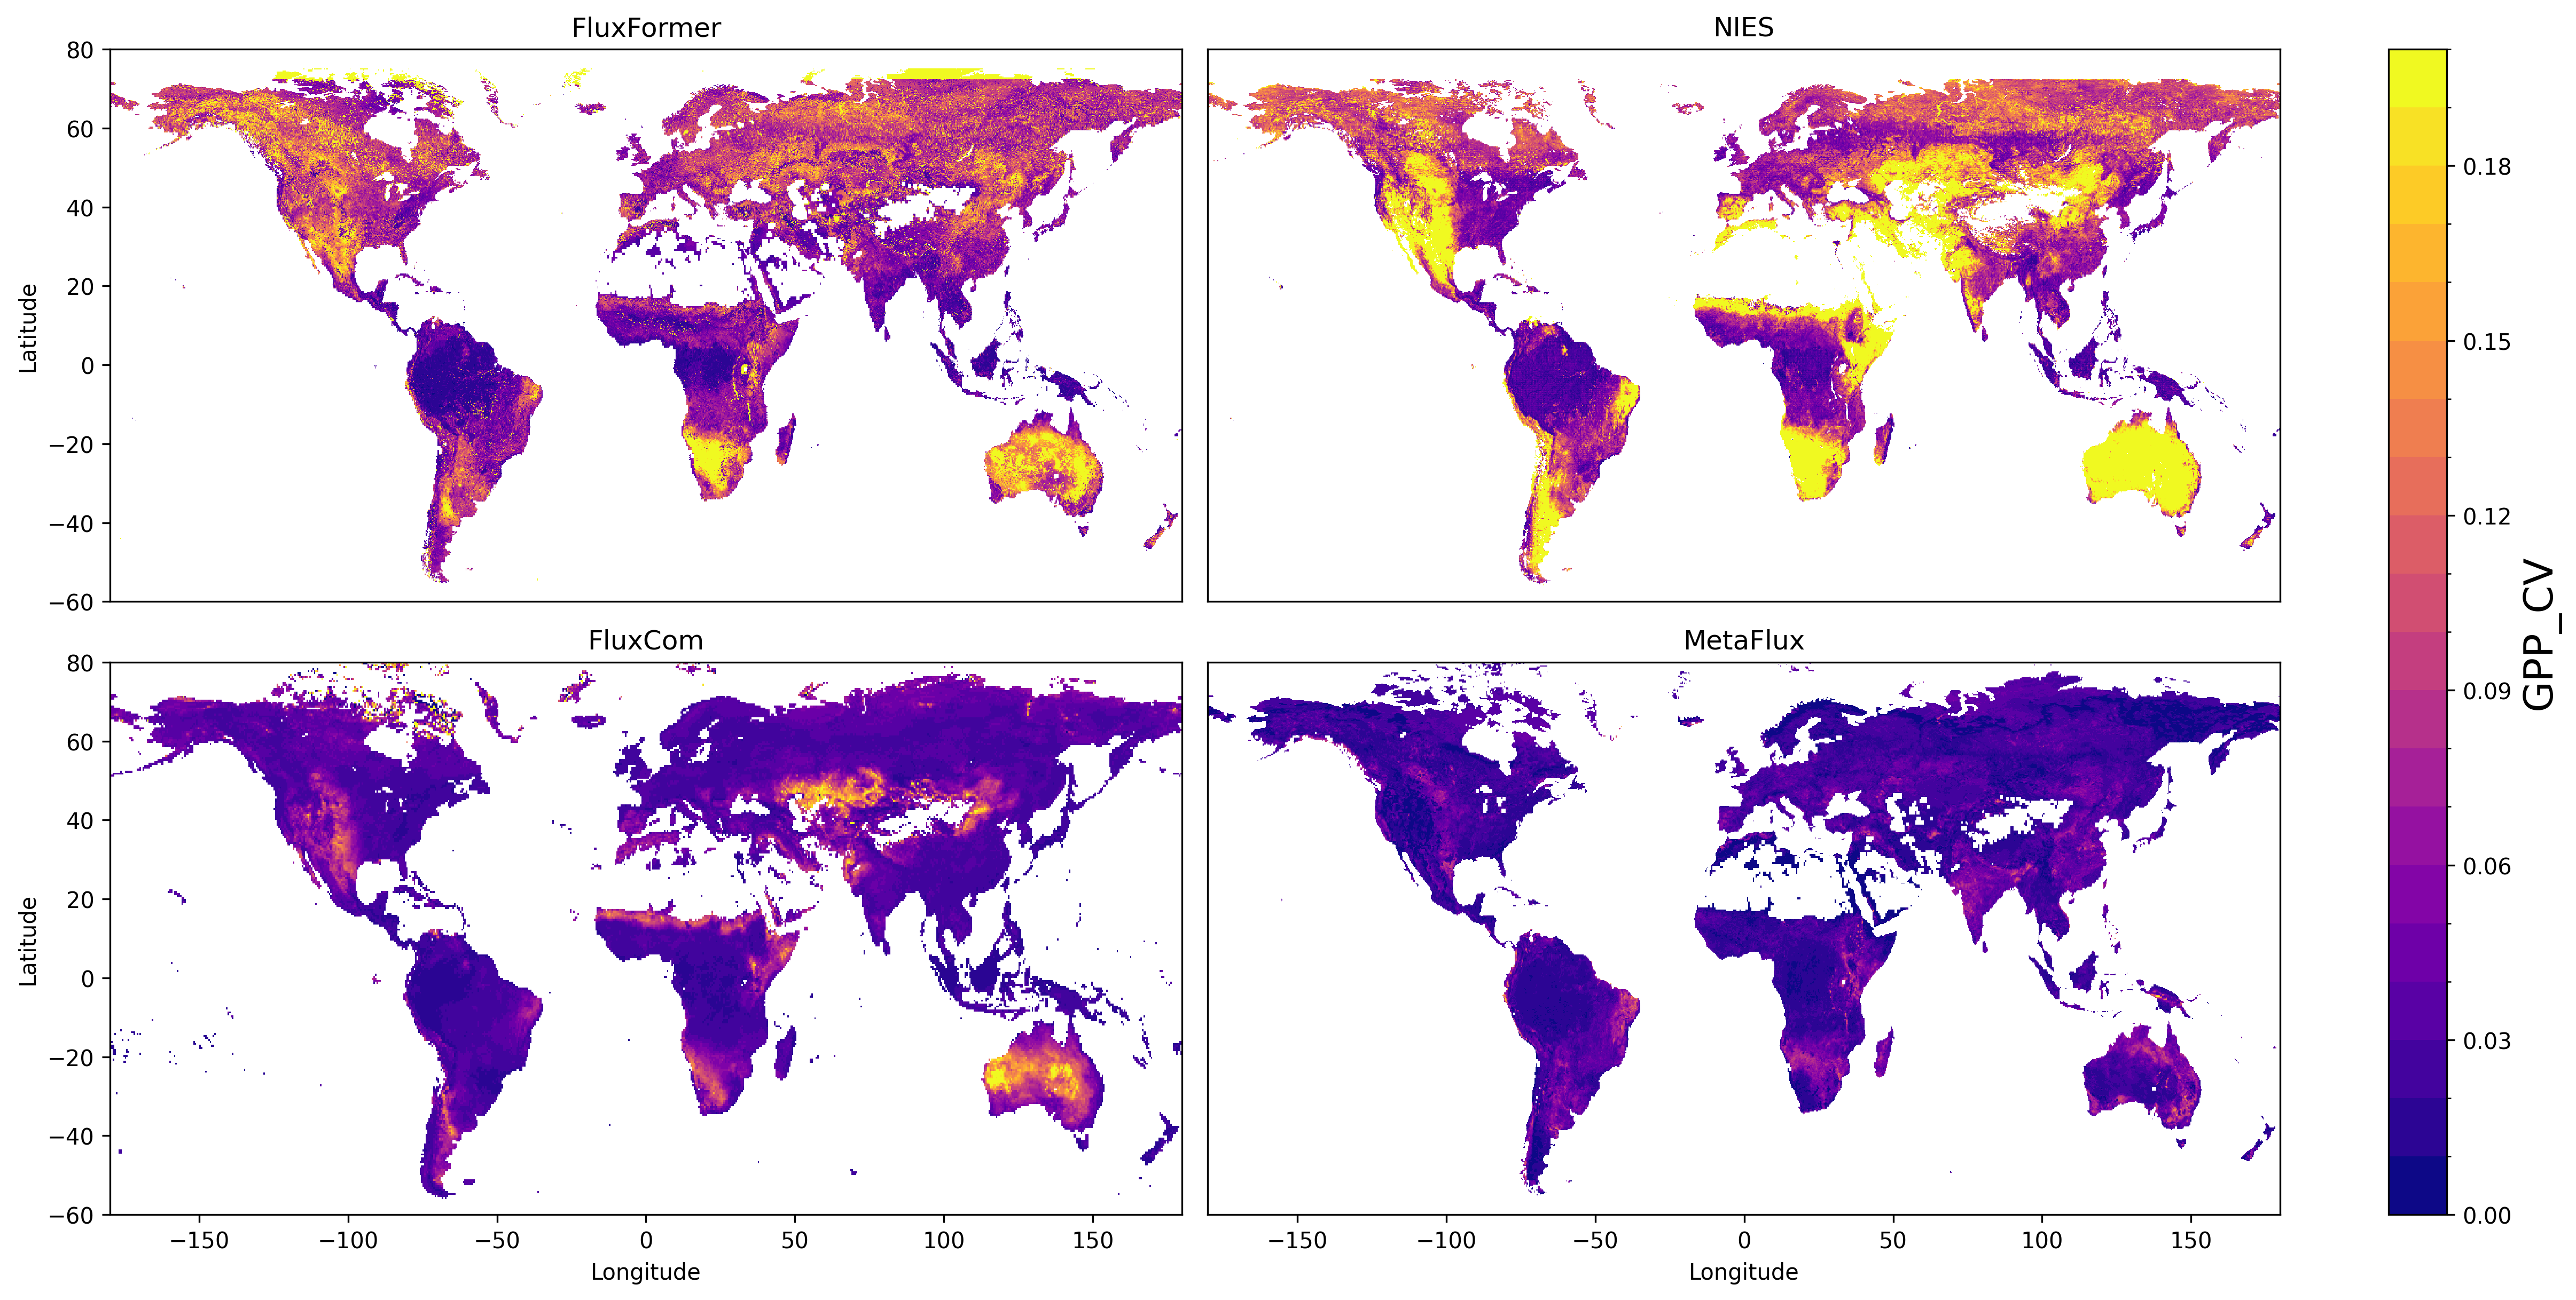
\includegraphics[width=\textwidth]{figs/chap6/IAV_GPP.png}
      \caption{GPP}
      \label{fig:chap6_fig8a}
    \end{subfigure}

    \begin{subfigure}{\textwidth}
      \centering
      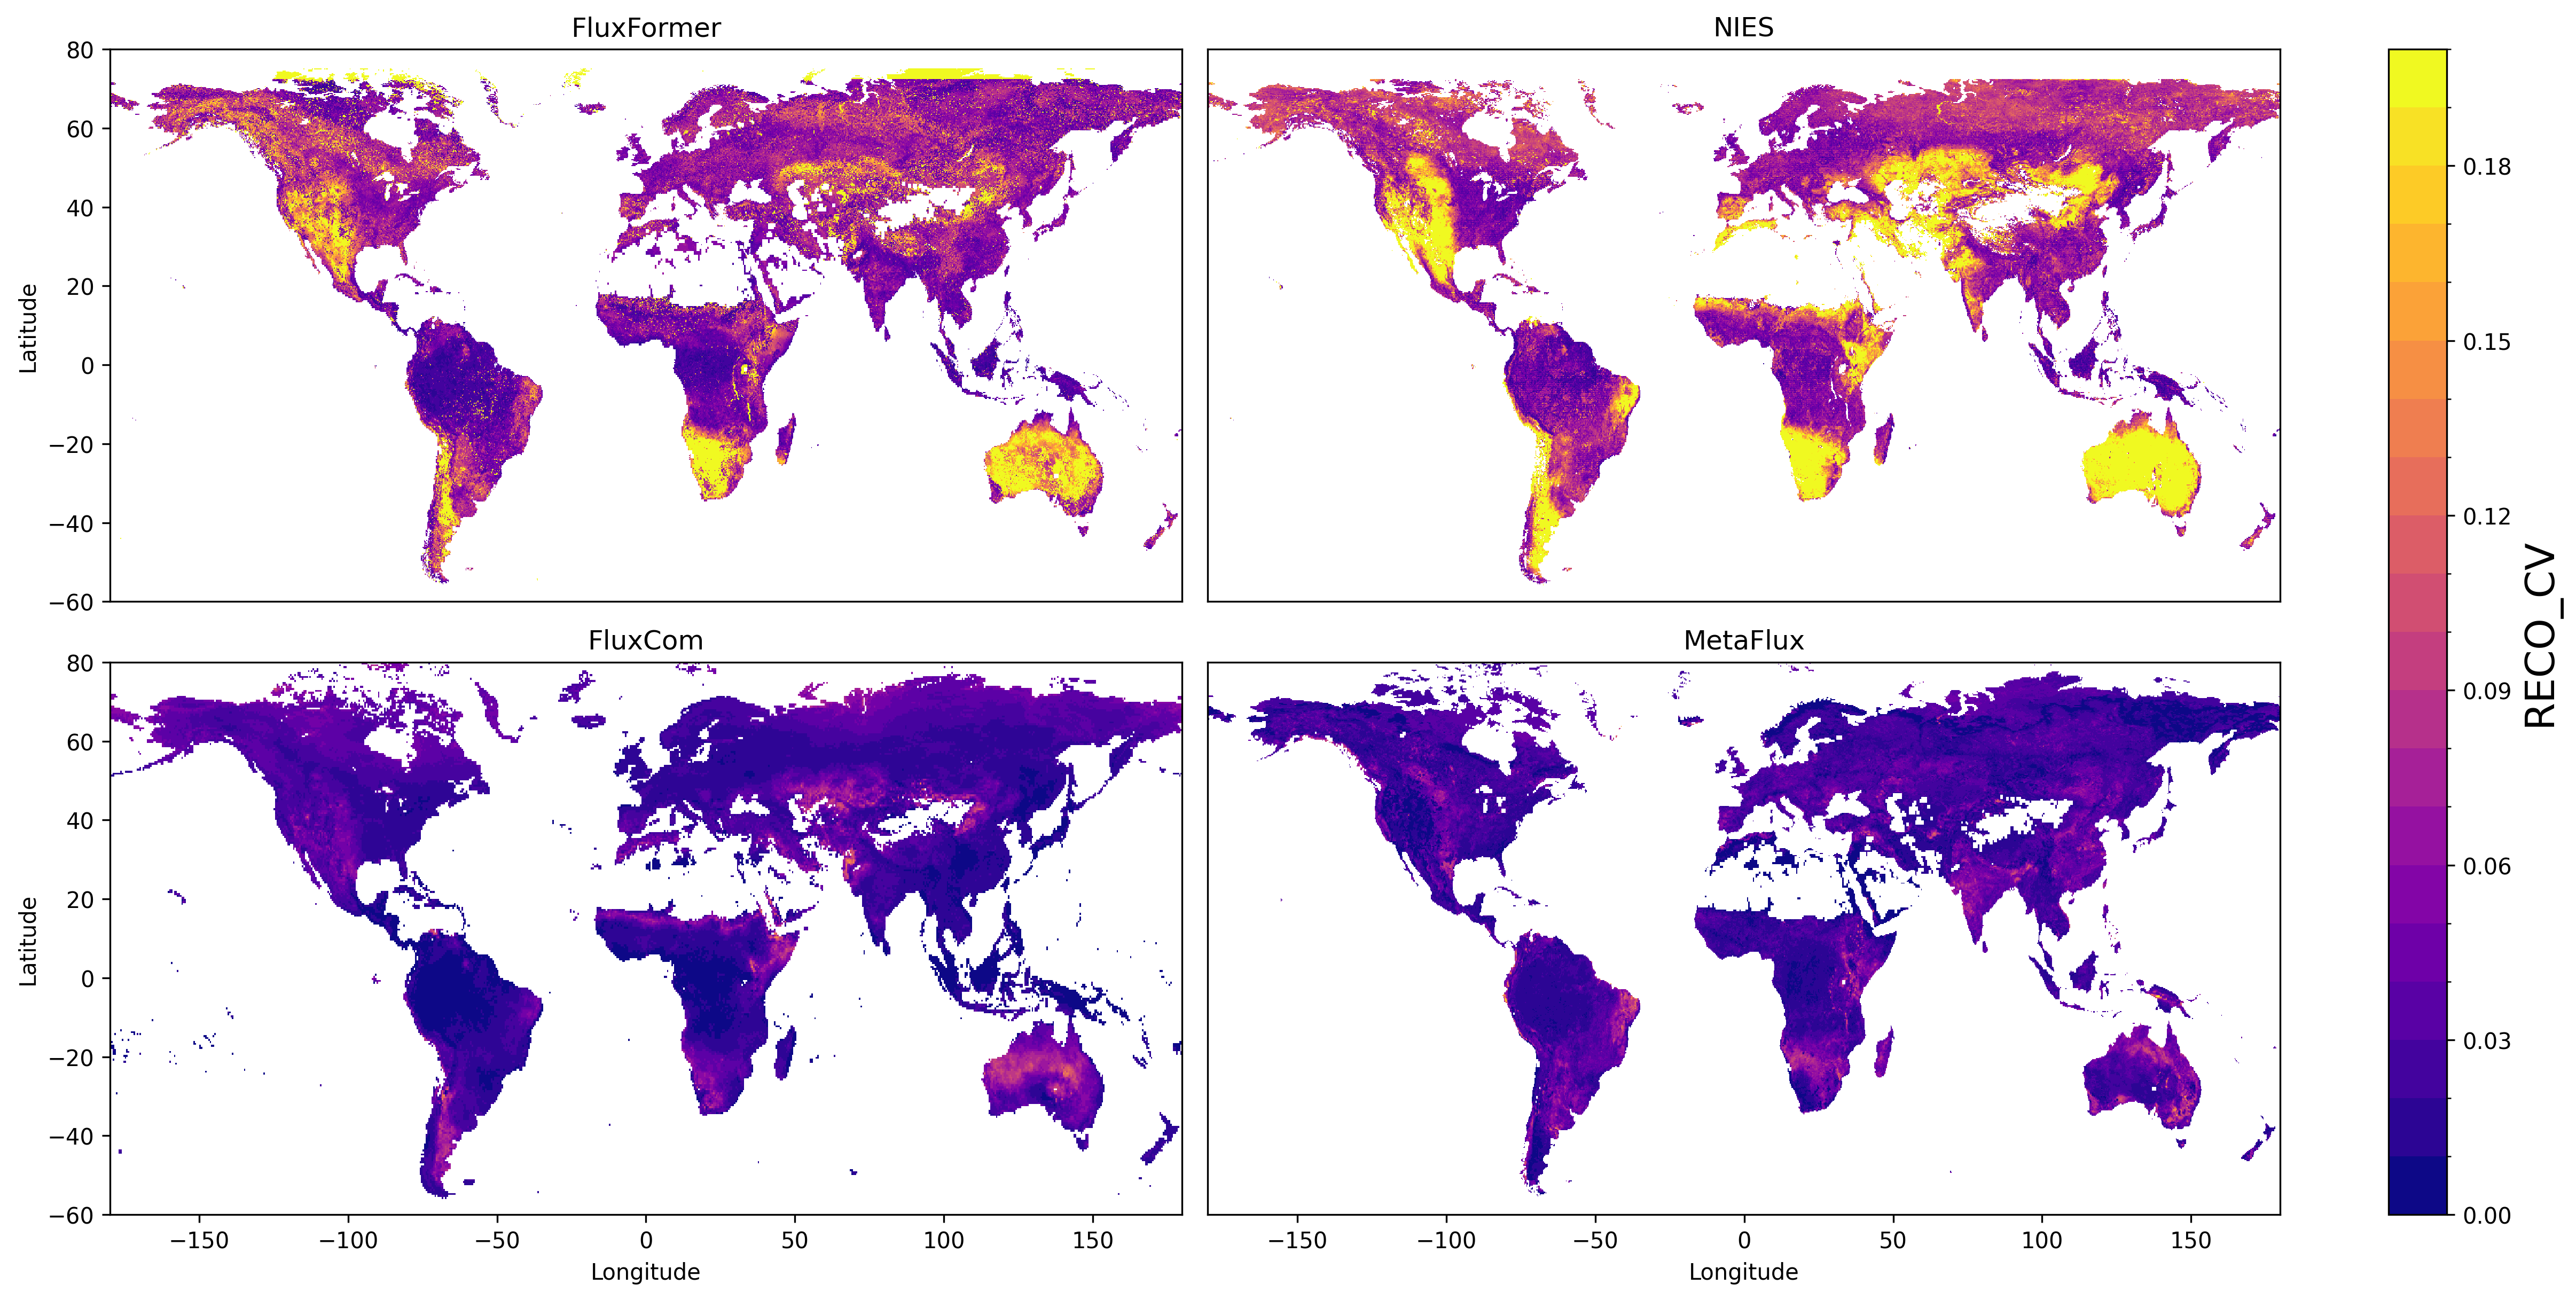
\includegraphics[width=\textwidth]{figs/chap6/IAV_RECO.png}
      \caption{RECO}
      \label{fig:chap6_fig8b}
    \end{subfigure}
    \caption{Interannual variations: GPP (a) RECO (b)}
    \label{fig:chap6_fig8}
\end{figure}